%%%%%%%%%%%%%%%%%%%%%%%%%%%%%%%%%%%%%%%%%%%%%%%%%%%%%%%%%%%%%%%%%%%%%%%%%%%%%%
%
% タイトル TeX用テンプレート 
% バージョン 2016-8-23 (Tu) 初版
% 作成者 北山天斗,剱崎健太郎
% 作成場所 金沢工業高等専門学校
% 用途 2段組レポートの作成等
%
%%%%%%%%%%%%%%%%%%%%%%%%%%%%%%%%%%%%%%%%%%%%%%%%%%%%%%%%%%%%%%%%%%%%%%%%%%%%%%%%
\documentclass[a4paper]{jarticle}
\usepackage{sice-si}
\usepackage{amsmath} 
\usepackage[dvipdfmx]{graphicx}

%%%%%%%%%%%%%%%%%%%%%%%%%%%%%%%%%%%%%%%%%%%%%%%%%%%%%%%%%%%%%%%%%%%%%%%%%%%%%%%%
\begin{document}\title{安全な研究用マルチコプターの開発}
\name{北山天斗,剱崎健太郎,伊藤恒平(金沢工業高等専門学校)}
\etitle{The development of safety multirotor for research}
\ename{Takato KITAYAMA,Kentro KENZAKI,Kouhei ITO(Kanazawa Technical College)}
\abst{
近年注目されているマルチコプターの研究開発に取り組む.
マルチコプターとは3つ以上のローターを持つ無人航空機である.
一般に流通しているものは4つのローターを持つマルチコプター(以下クアッドコプター)である.
ローターが4つであると,前後左右の姿勢制御がイメージしやすい.
そのため本研究では4つのローターを持つクアッドコプターの研究開発を行う.
}

\maketitle
%%%%%%%%%%%%%%%%%%%%%%%%%%%%%%%%%%%%%%%%%%%%%%%%%%%%%%%%%%%%%%%%%%%%%%%%%%%%%%%%
\section{はじめに}

\subsection{研究の背景}
近年注目されているマルチコプターであるが,開発に取り組まれているのは屋外向けのものが主である.
例えば大手通販企業amazonではマルチコプターを使った宅配システムなどが開発されている.
また,テレビ番組でもマルチコプターを使用して撮影された映像が時折放送されている.
しかし,マルチコプターは屋内での使用用途が少ないため屋内向けマルチコプターはあまり注目されていない.
本研究ではそこに注目し屋内向けマルチコプターの用途を見つけ出し,その用途に適した機体とプログラムの研究開発を行う.
また,マルチコプターのプロペラに巻き込まれて怪我をするという事故が多く見受けられる.
特に屋内であればマルチコプターと人間の距離が近くなるため,一層安全性の向上が必要となる.
これを未然に防ぐため,機体を覆うものを取り付け安全性の向上を試みる.

\subsection{研究の目的}
前述の理由から屋内においてマルチコプターでできることを挙げ,その目標を達成するために必要なハードウェア,ソフトウェアの開発に取り組む.

本研究室では屋外自律移動ロボットの開発するために単眼カメラを用いた三次元復元,マッピングシステムの開発が行われた.
そのシステムの使用にはカメラの移動が必要不可欠である.
マルチコプターであれば前後左右だけでなく上下にも自由に動くことができるため,このシステムの使用に適している.
そこでマルチコプターにこのシステムを搭載し,指定した始点と終点までの間の3次元マッピングを自動で行うことを目的として研究開発を行う.

\subsection{本稿の構成}
本論文は前半でハードウェア開発,後半でソフトウェア開発について述べる.

%%%%%%%%%%%%%%%%%%%%%%%%%%%%%%%%%%%%%%%%%%%%%%%%%%%%%%%%%%%%%%%%%%%%%%%%%%%%%%%

\section{ハードウェア開発の目標}
自作マルチコプターは2段階の分けて製作を行う.
1段階目では機体の耐久性や組み立て易さなどを考慮し,機体の形状を決定する.
2段階目ではマルチコプターのプロペラに巻き込まれて怪我をする事故の防止と落下時の衝撃から機体を保護するため機体を球体で覆う.

\subsection{機体の設計製作}
アルミ製のアームと樹脂製の取付板,RaspberryPi3(以下RPi)とNavio2、T-MOTOR製のモーター・ESC・プロペラを用いて機体を設計製作する.

\subsection{球体}
機体の大きさから外径510mm内径450mmとなるように輪状のスチレンボードを組み立てて半球を2つ作り,組み合わせて機体を覆う.
CADで作成した球体のイメージをFig.\ref{fig:sphere-CAD}に示す.

\begin{figure}[htbp]
 \begin{center}
  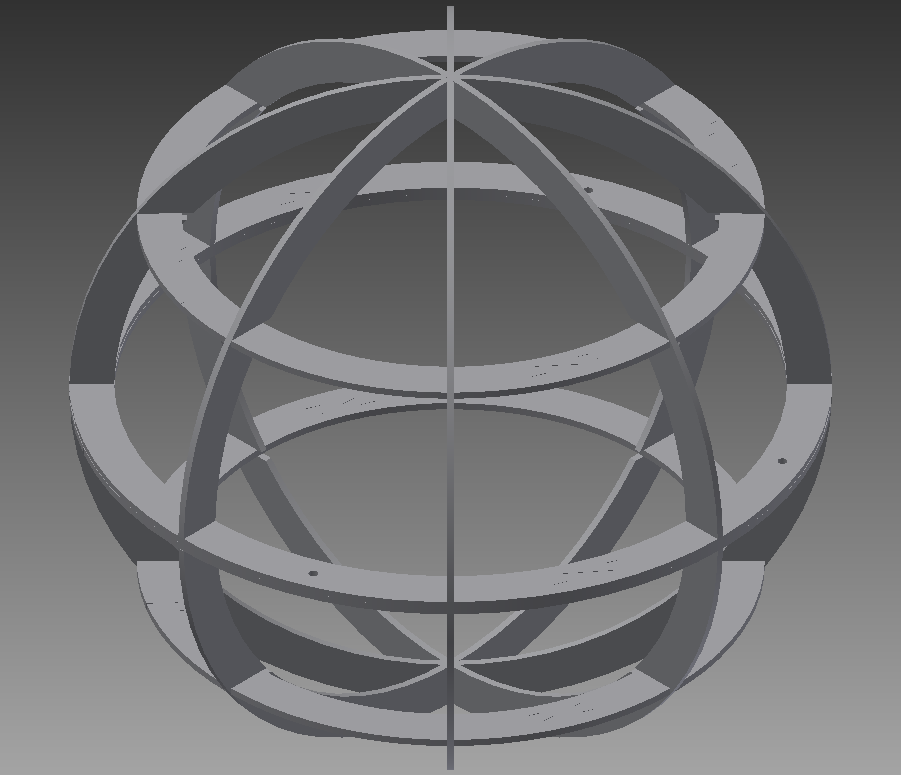
\includegraphics[width=50mm]{image/sphere-CAD.png}
  \caption{球体イメージ}
  \label{fig:sphere-CAD}
 \end{center}
\end{figure}

\section{ハードウェア開発の経緯}

\subsection{本体}

\subsubsection{試作1号機}
はじめに試作1号機として,80mm×80mm,厚さ2mmのアルミ角管を高さ20mmに切断し各面にアームを取り付けたものを試作した.
実際に製作した試作1号機をFig.\ref{fig:drone-1},球体1号機と組み合わせた球体マルチコプター1号機をFig.\ref{fig:1}に示す.
また球体と組み合わせた際の重量は750gであった.
この試作1号機では、アームの縦方向の荷重に対する強度やバッテリーなどの取り付け位置・方法が問題となったため,改善の必要がある.

\begin{figure}[htbp]
 \begin{center}
  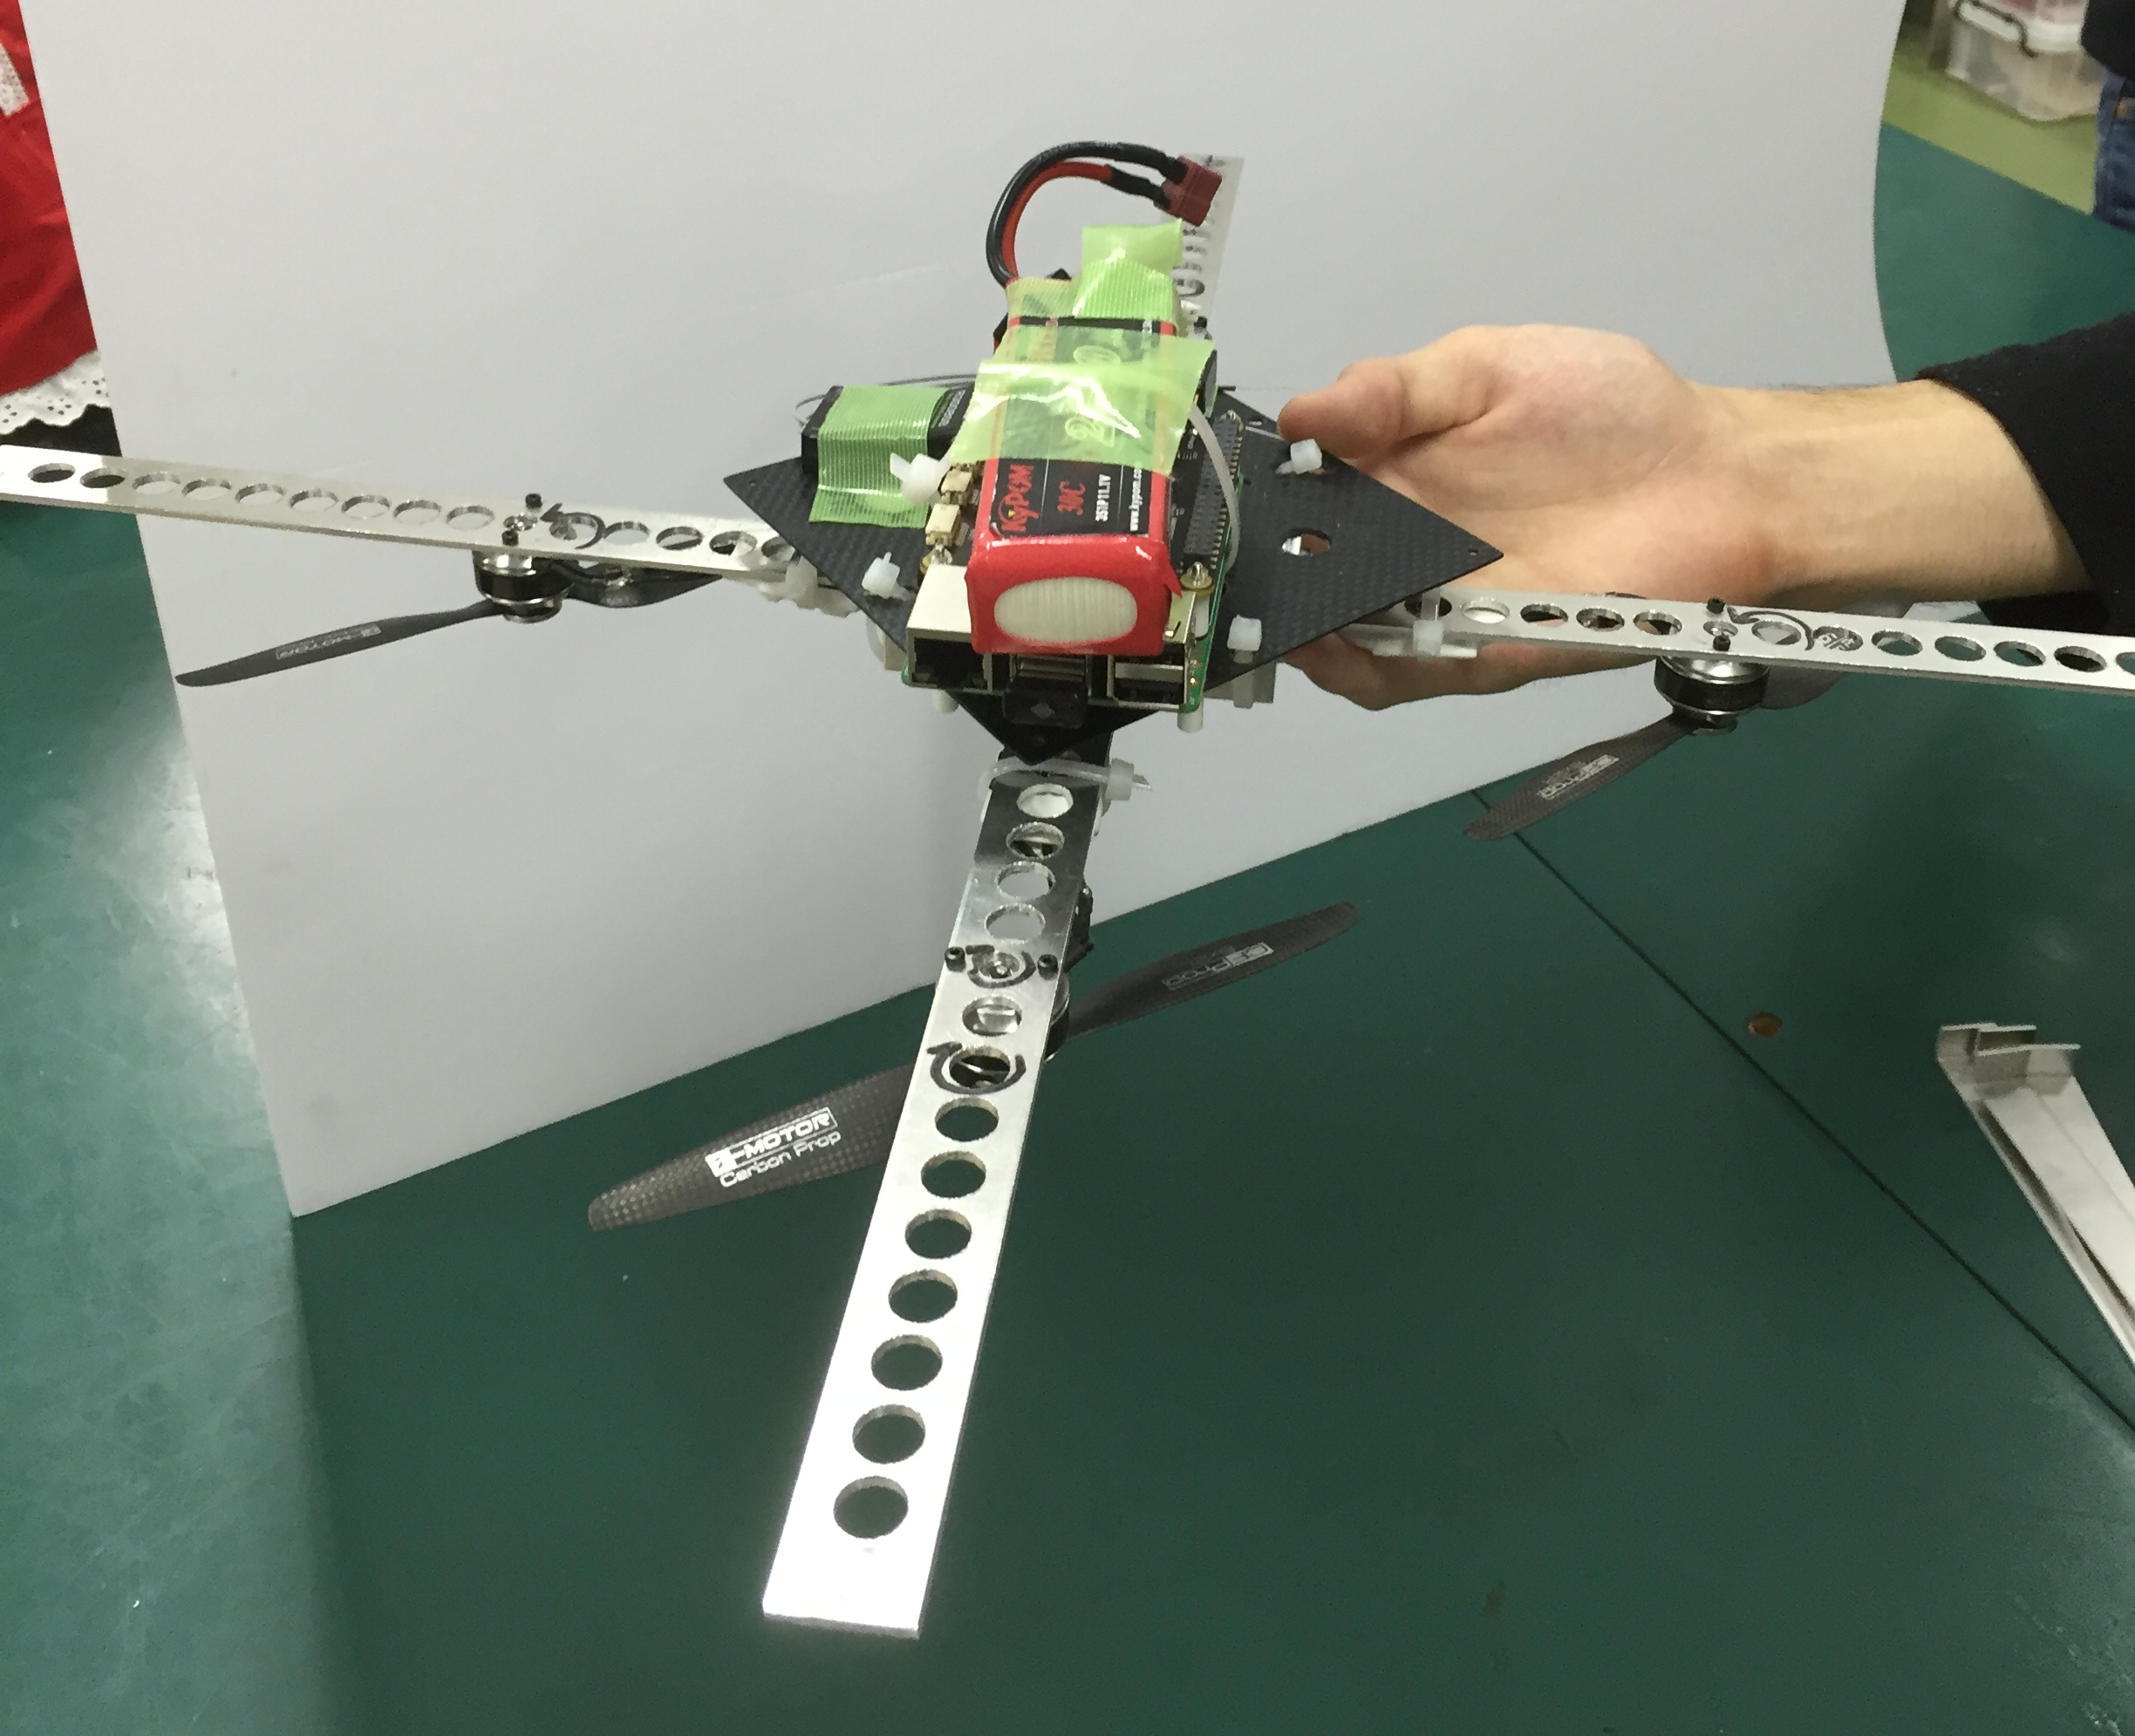
\includegraphics[width=50mm]{image/multirotor-1.JPG}
  \caption{試作機1号機}
  \label{fig:drone-1}
 \end{center}
\end{figure}

\begin{figure}[htbp]
 \begin{center}
  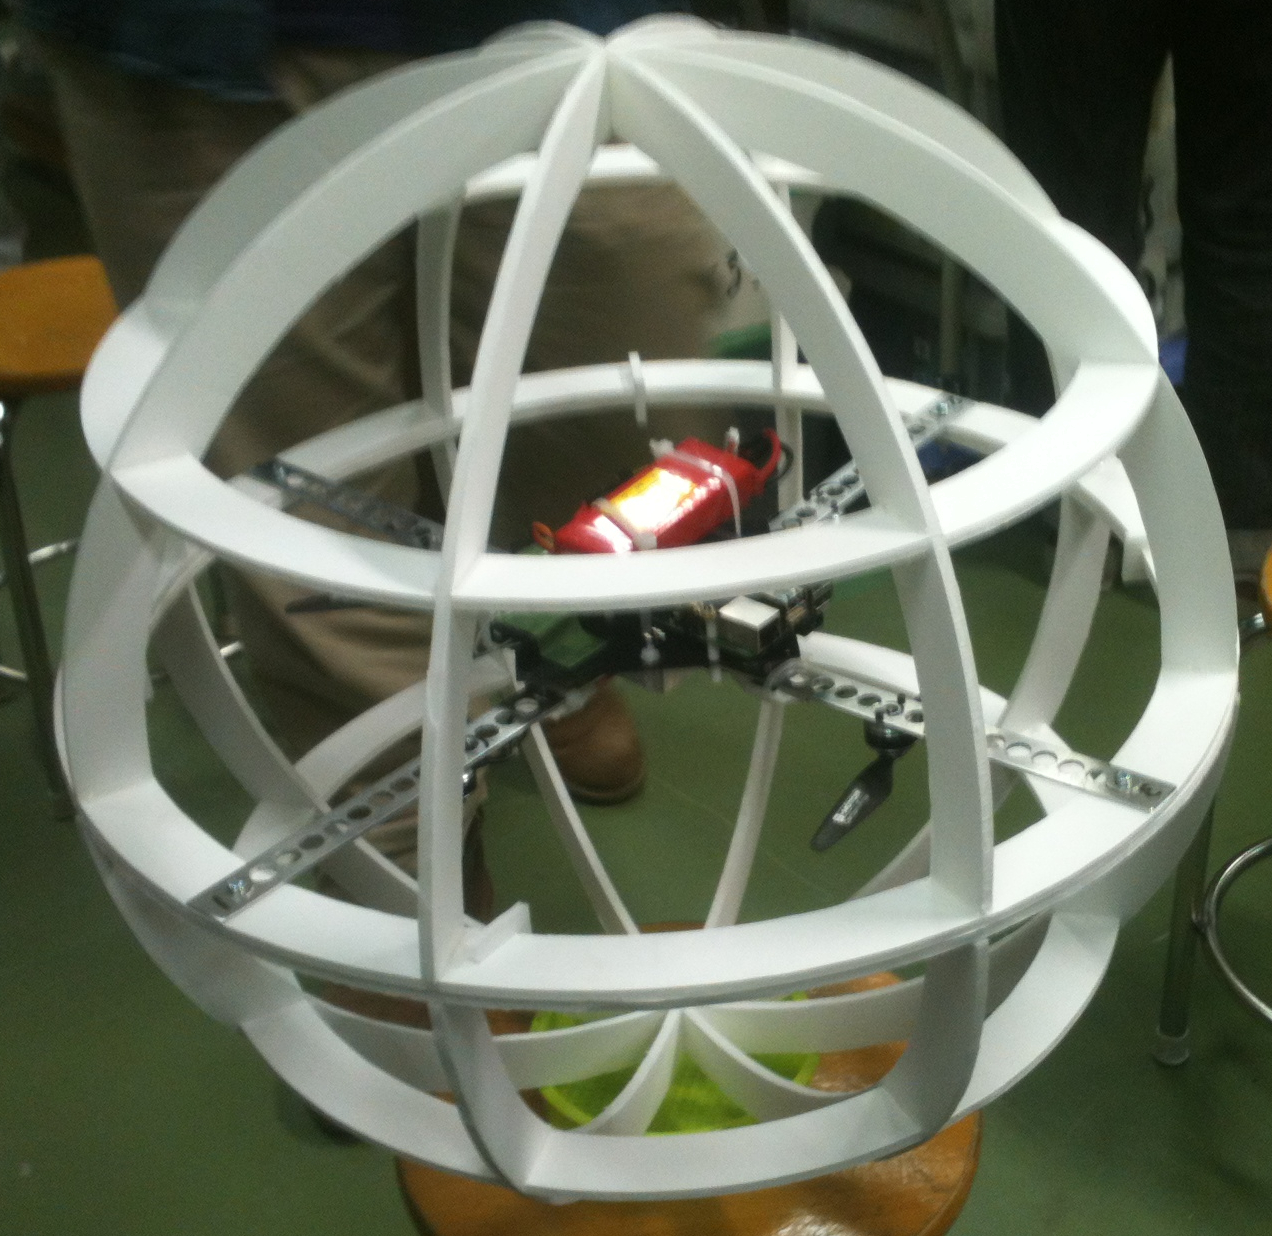
\includegraphics[width=50mm]{image/1.JPG}
  \caption{球体マルチコプター2号機}
  \label{fig:1}
 \end{center}
\end{figure}

\subsubsection{試作2号機、3号機}
試作1号機での問題点を改良し,試作2号機と3号機を同時に製作した.
アームの縦方向の荷重に対する強度は,25mm×15mm、厚さ1.5mmのアルミ角管を半分に切断したコの字型のものをFig.\ref{fig:arm}のように交差させたものに変更することで改良した.
バッテリーの取り付け位置・方法は,ABS樹脂板をレーザー加工機で加工することでFig.\ref{fig:RPi-board}のような専用の取付板を製作して改良を行った.
試作3号機と球体3号機を組み合わせた球体マルチコプター3号機をFig.\ref{fig:3}に示す.3号機の重量は約716gで1号機と比較して35g程度の軽量化ができた.

\begin{figure}[htbp]
 \begin{center}
  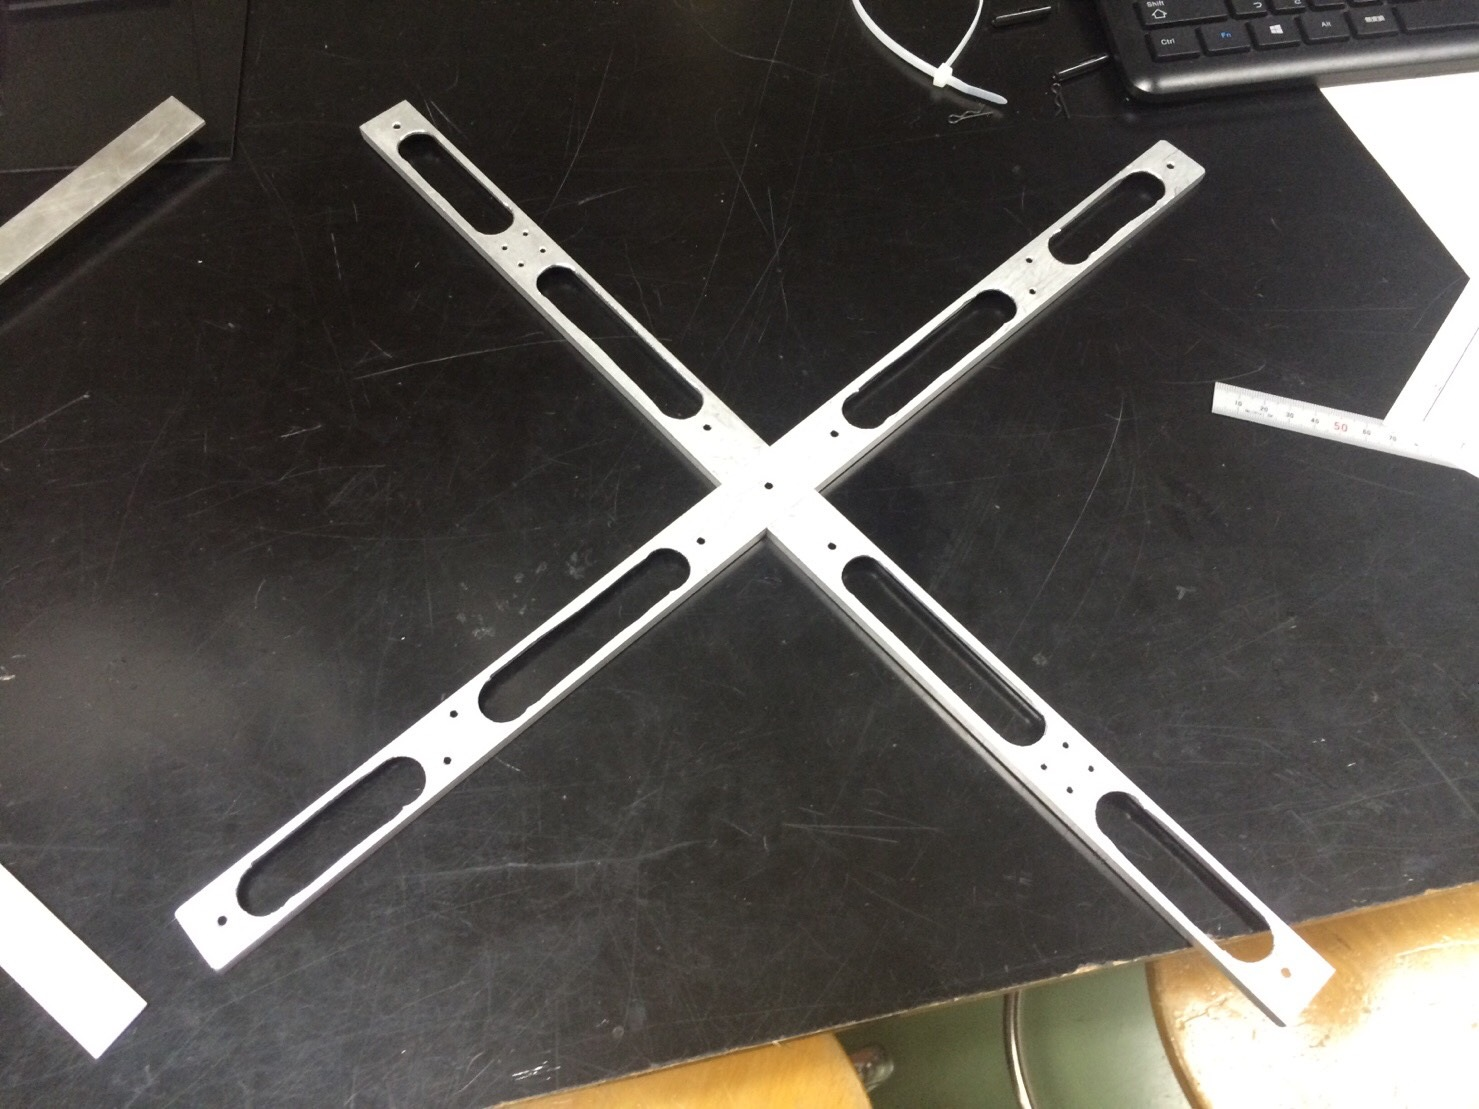
\includegraphics[width=50mm]{image/arm-2.JPG}
  \caption{改良したアーム}
  \label{fig:arm}
 \end{center}
\end{figure}

\begin{figure}[htbp]
 \begin{center}
  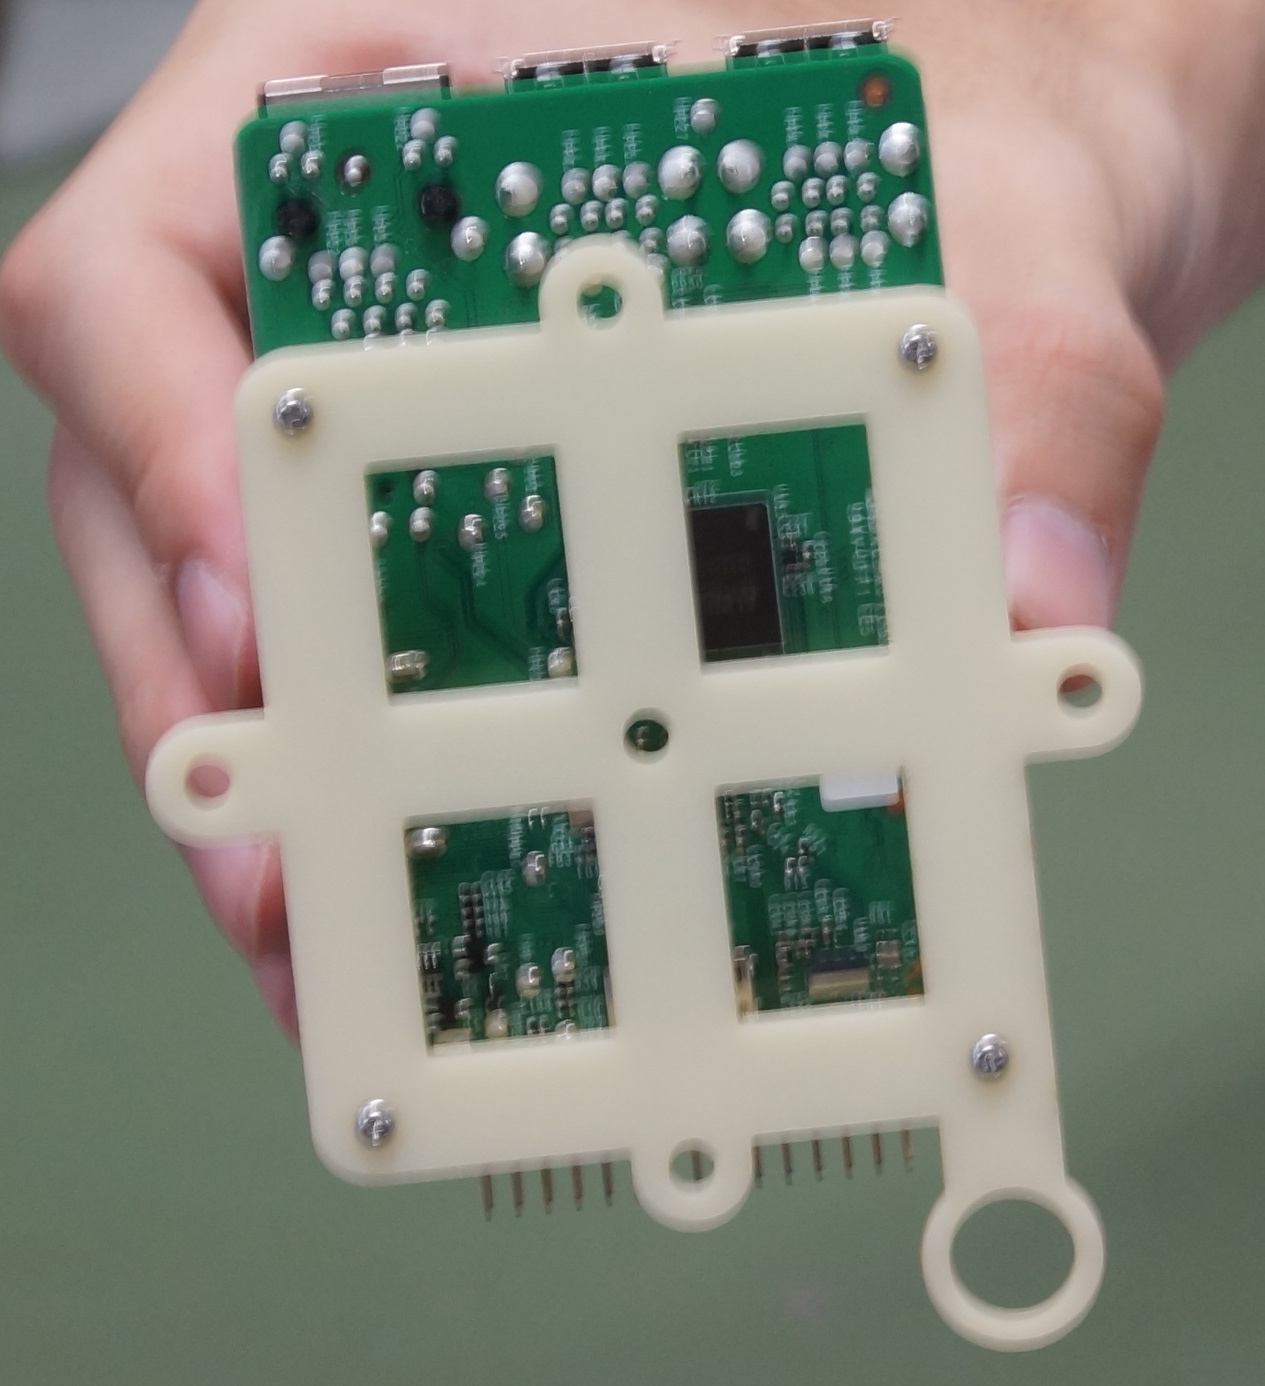
\includegraphics[width=50mm]{image/RPi-board-1.JPG}
  \caption{RPi取付板}
  \label{fig:RPi-board}
 \end{center}
\end{figure}

\begin{figure}[htbp]
 \begin{center}
  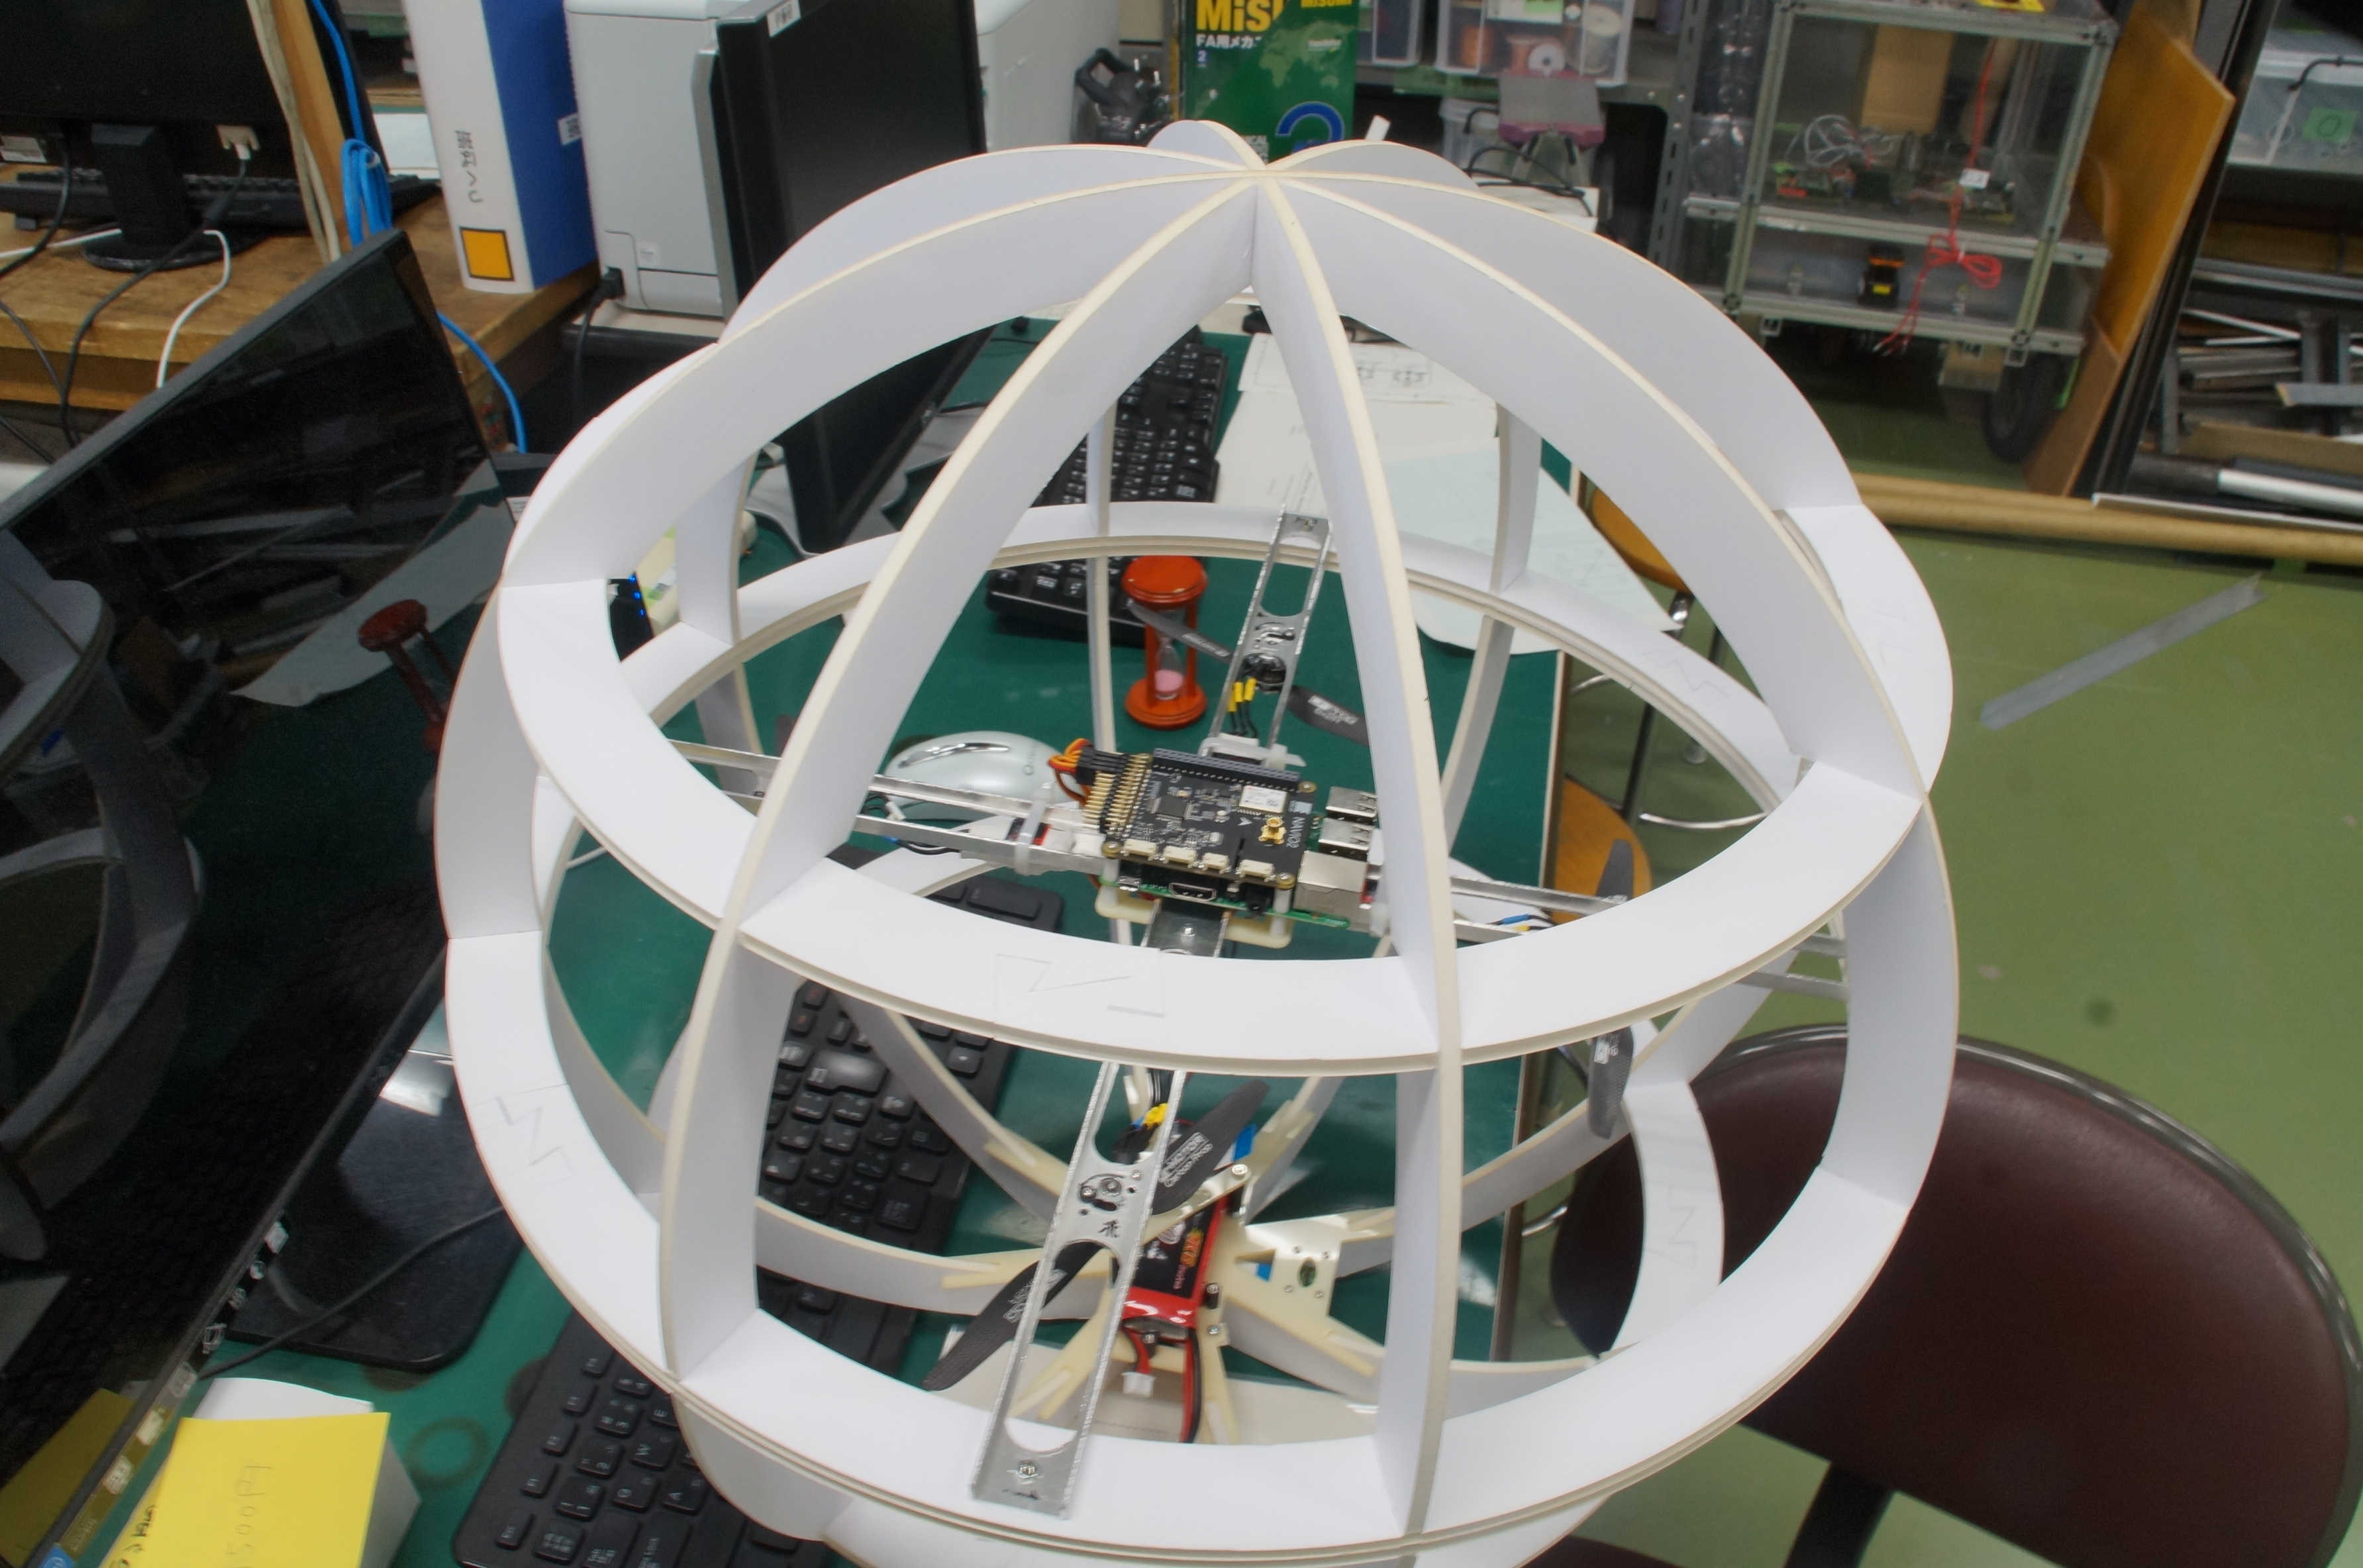
\includegraphics[width=50mm]{image/3.JPG}
  \caption{球体マルチコプター3号機}
  \label{fig:3}
 \end{center}
\end{figure}

\subsubsection{制御実験機1号機}
球体2号機,3号機はスチレンボードの強度が弱く,落下により大破する事案が発生した(後述).
そのため,プログラムによる制御の安定化がある程度実現できるまでの実験機として,制御実験機1号機を製作した.
試作2号機の本体をベースとして各アーム先端と機体中央下部に足を取り付け,最低限の安全性を確保するためプラスチックダンボールの輪を取り付けたメンテナンスが容易なものを製作した.
製作した制御実験機1号機をFig.\ref{fig:test-machine-1}に示す.

足があるため離着陸が容易なため,制御実験を行う上では非常に扱いが容易であった.
中央下部にも足を取り付けていたが着地の衝撃が予想以上に強く,アーム中央が沈むように歪んだ.

\begin{figure}[htbp]
 \begin{center}
  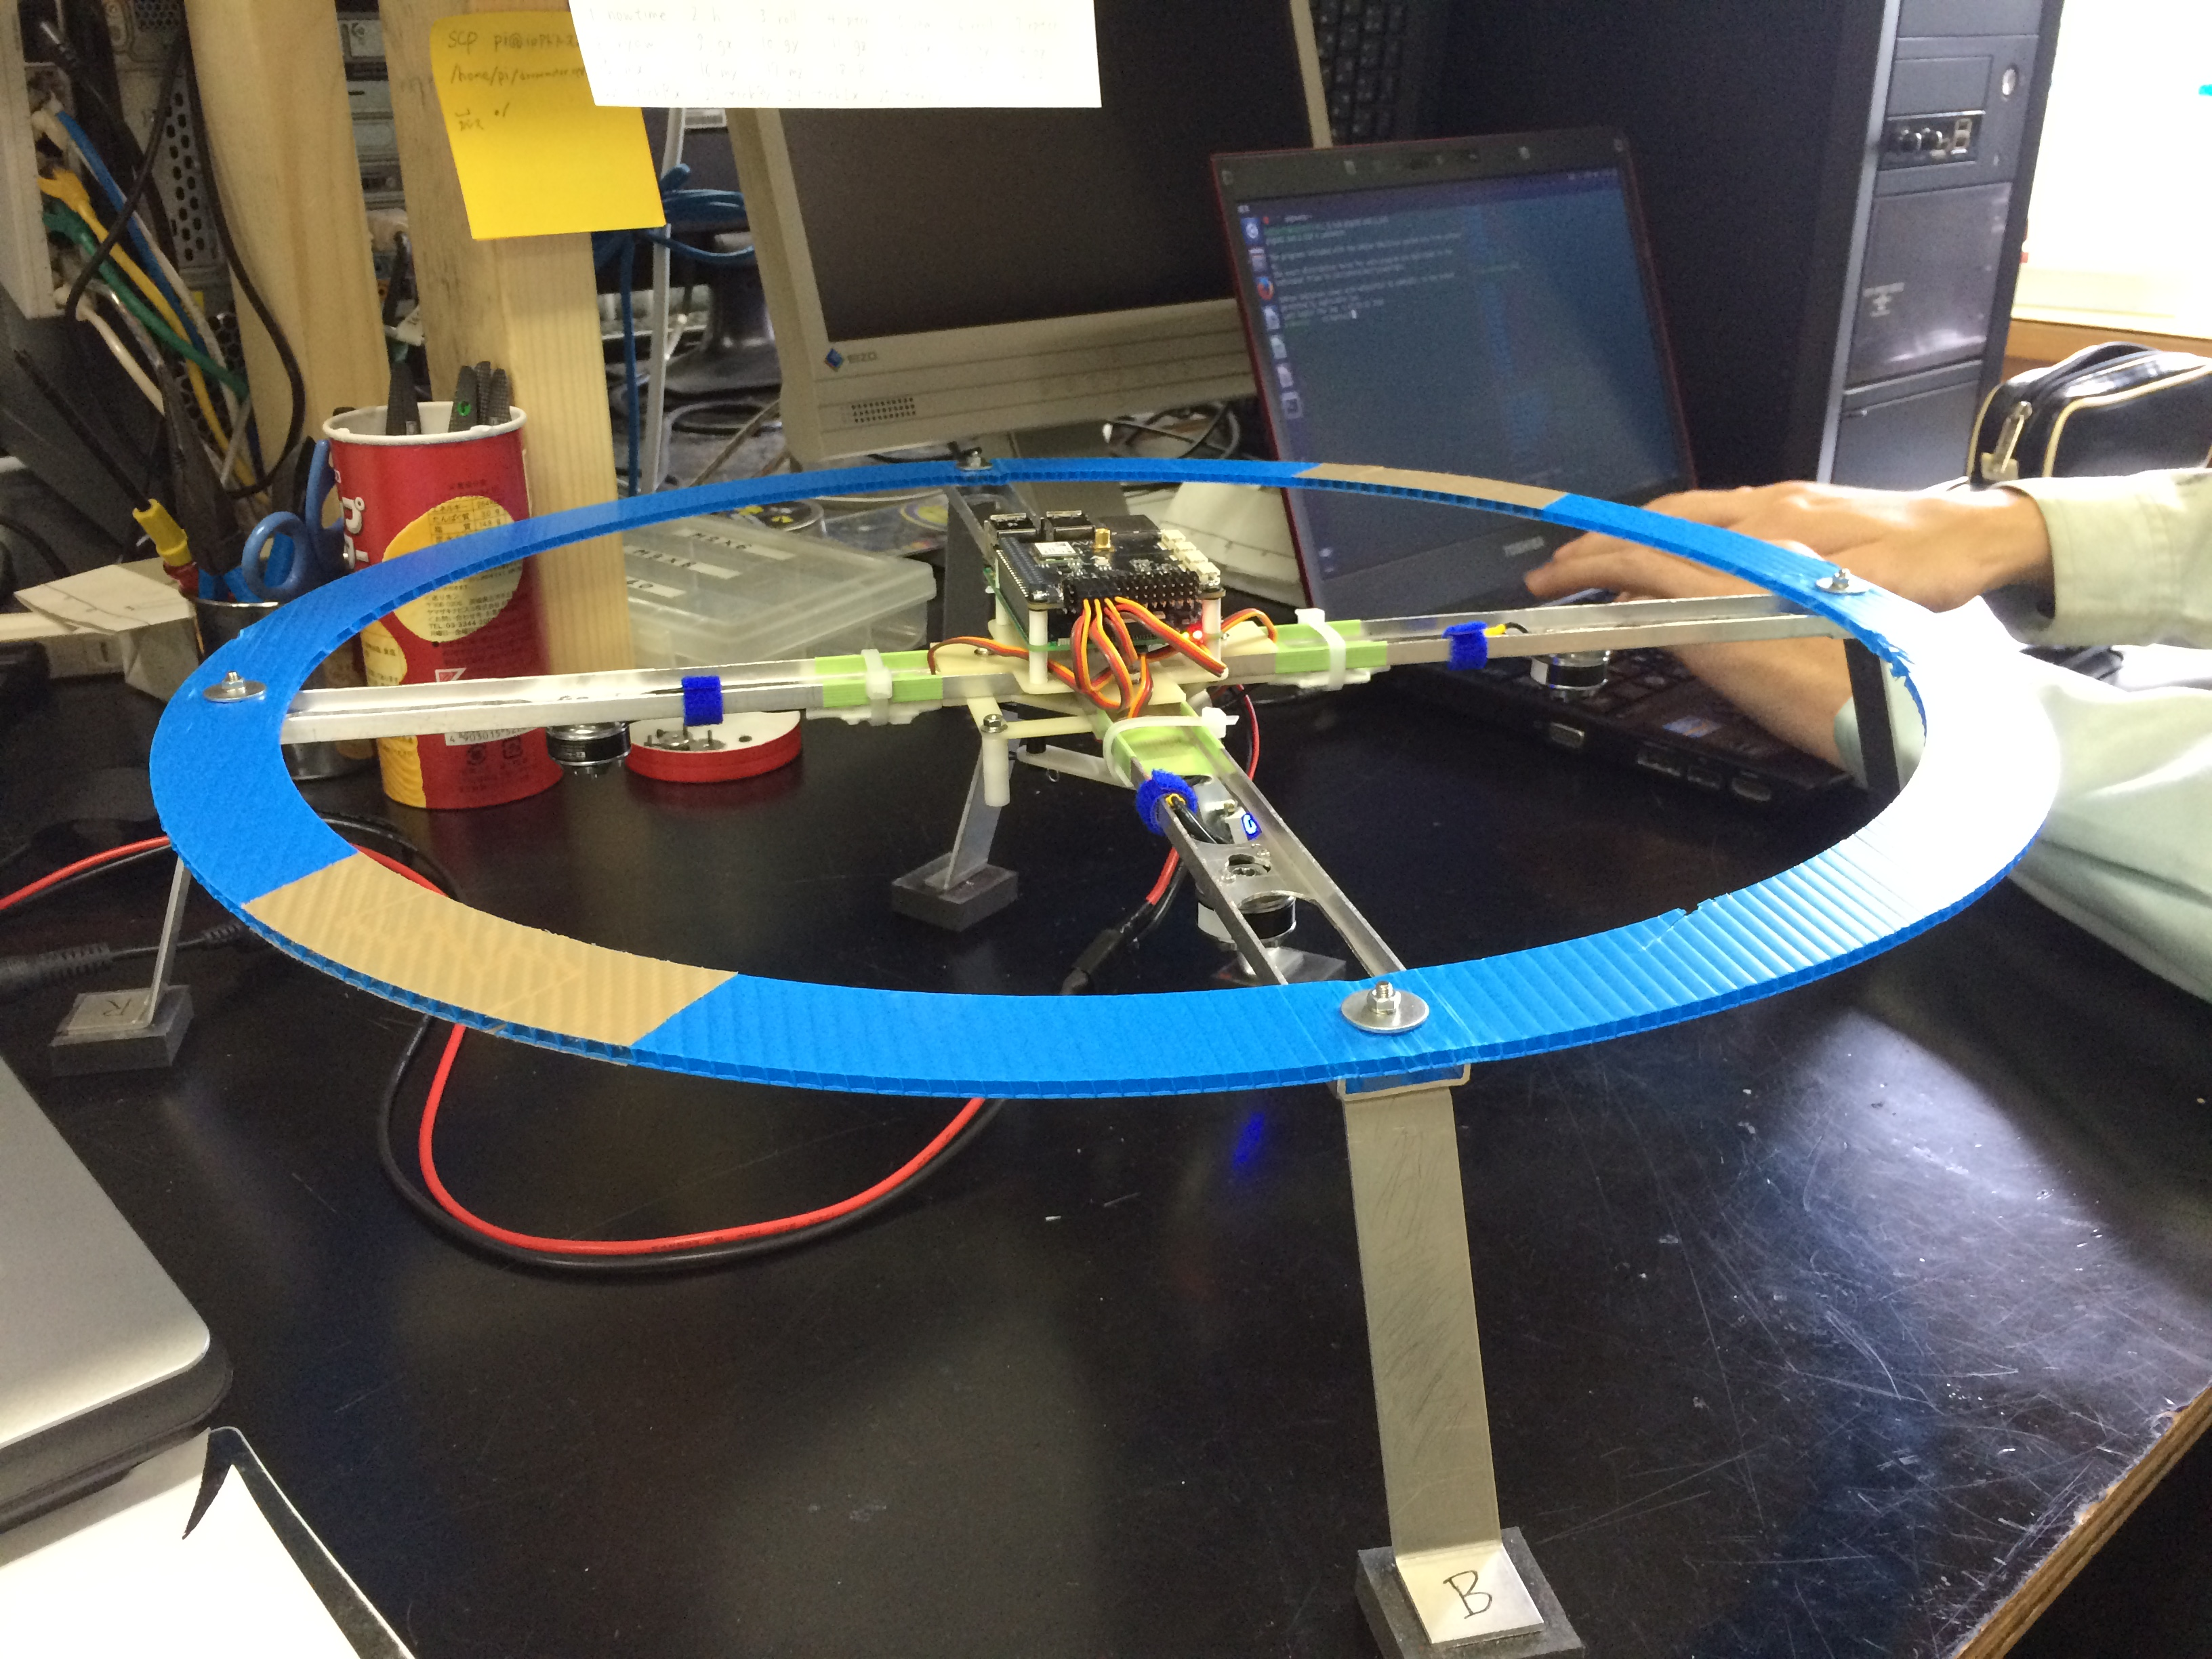
\includegraphics[width=50mm]{image/test-machine-1.JPG}
  \caption{制御実験機1号機}
  \label{fig:test-machine-1}
 \end{center}
\end{figure}

\subsubsection{制御実験機2号機}
研究室にあった直径12mmのCFRP(Carbon Fiber Reinforced Plastics:炭素繊維強化プラスチック)のパイプを利用して新しい機体を開発した.
各アームに2本のパイプを使用し,中央で固定用パーツで上下から挟み込んで固定する.
またモーターの取り付け位置等にはパイプ間に板を取り付ける.
アームの材料の違いから軽量化が見込まれていたが,固定パーツが重く全体の重量は増加してしまった.
製作した本機体1号機をFig.\ref{fig:test-machine-2}に示す.

\begin{figure}[htbp]
 \begin{center}
  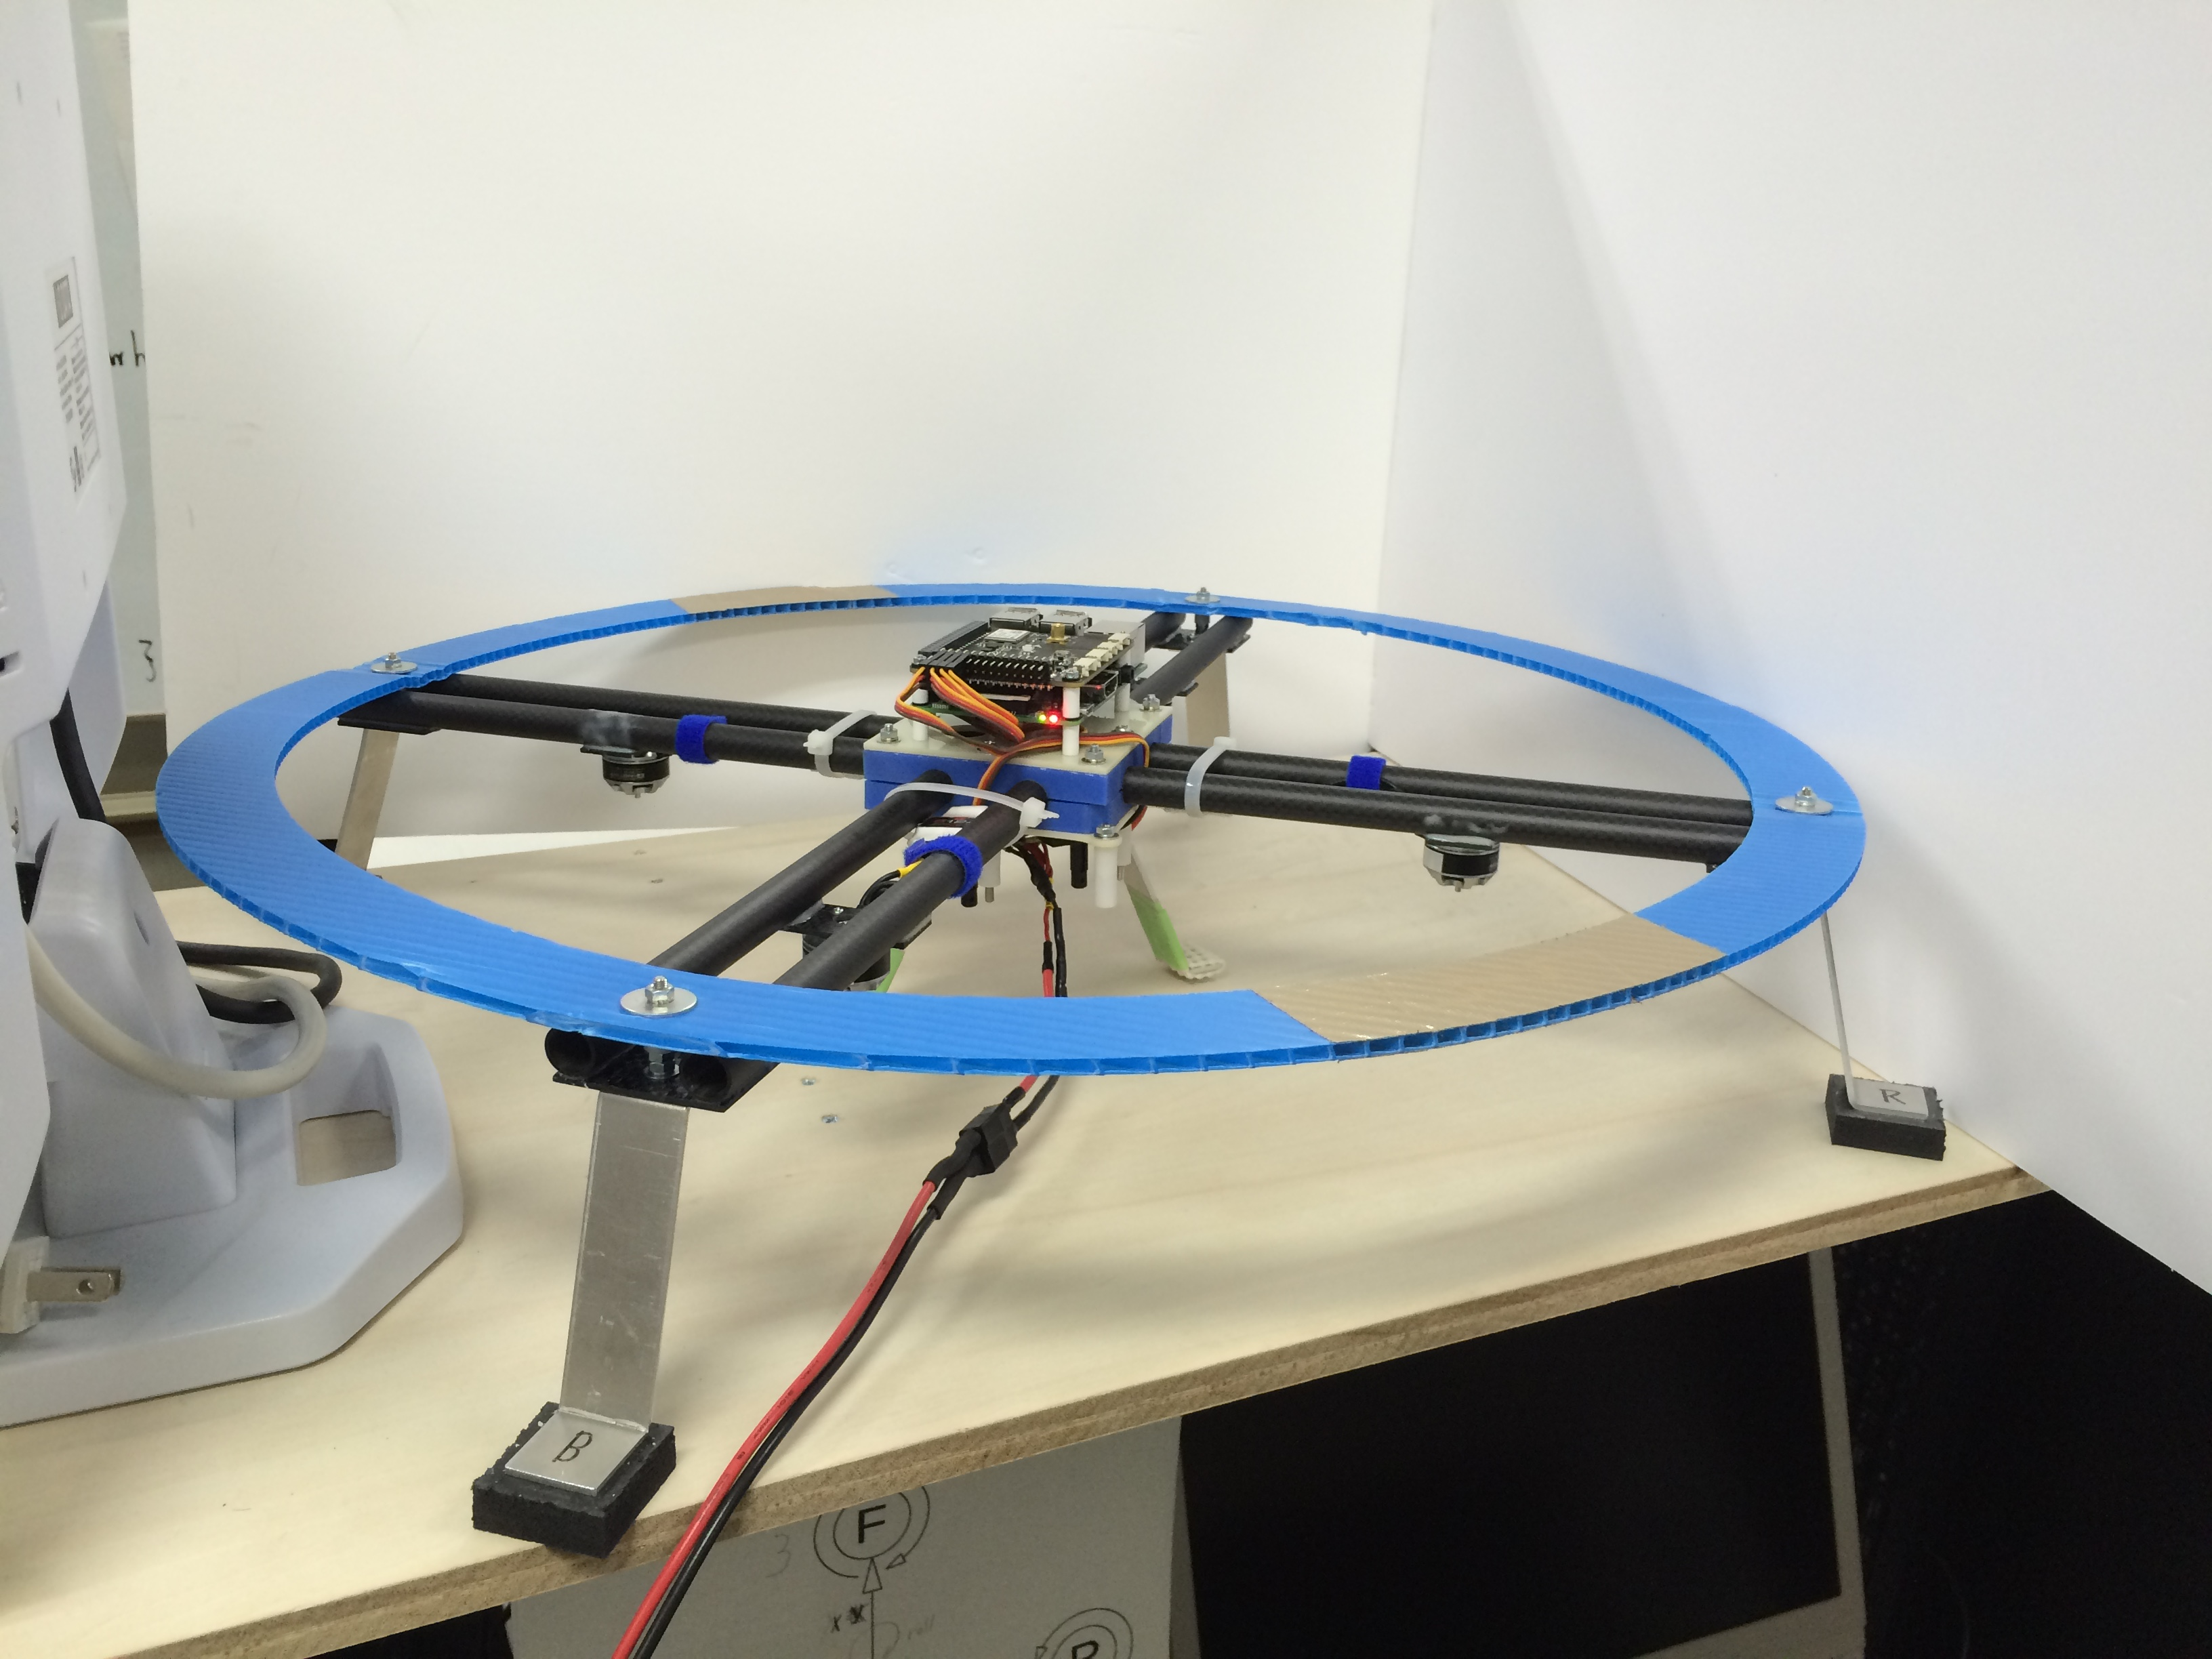
\includegraphics[width=50mm]{image/test-machine-2.JPG}
  \caption{制御実験機2号機}
  \label{fig:test-machine-2}
 \end{center}
\end{figure}

\subsection{球体}

\subsubsection{1号機}
輪状のスチレンボードを分割し,スチのり(酢酸ビニル樹脂系接着剤)で接着して組み立てた.
製作した球体1号機をFig.\ref{fig:sphere-1}に示す.
幾度か使用していると接合部のスチレンボードの紙がスチレン材から剥がれてしまった.

\begin{figure}[htbp]
 \begin{center}
  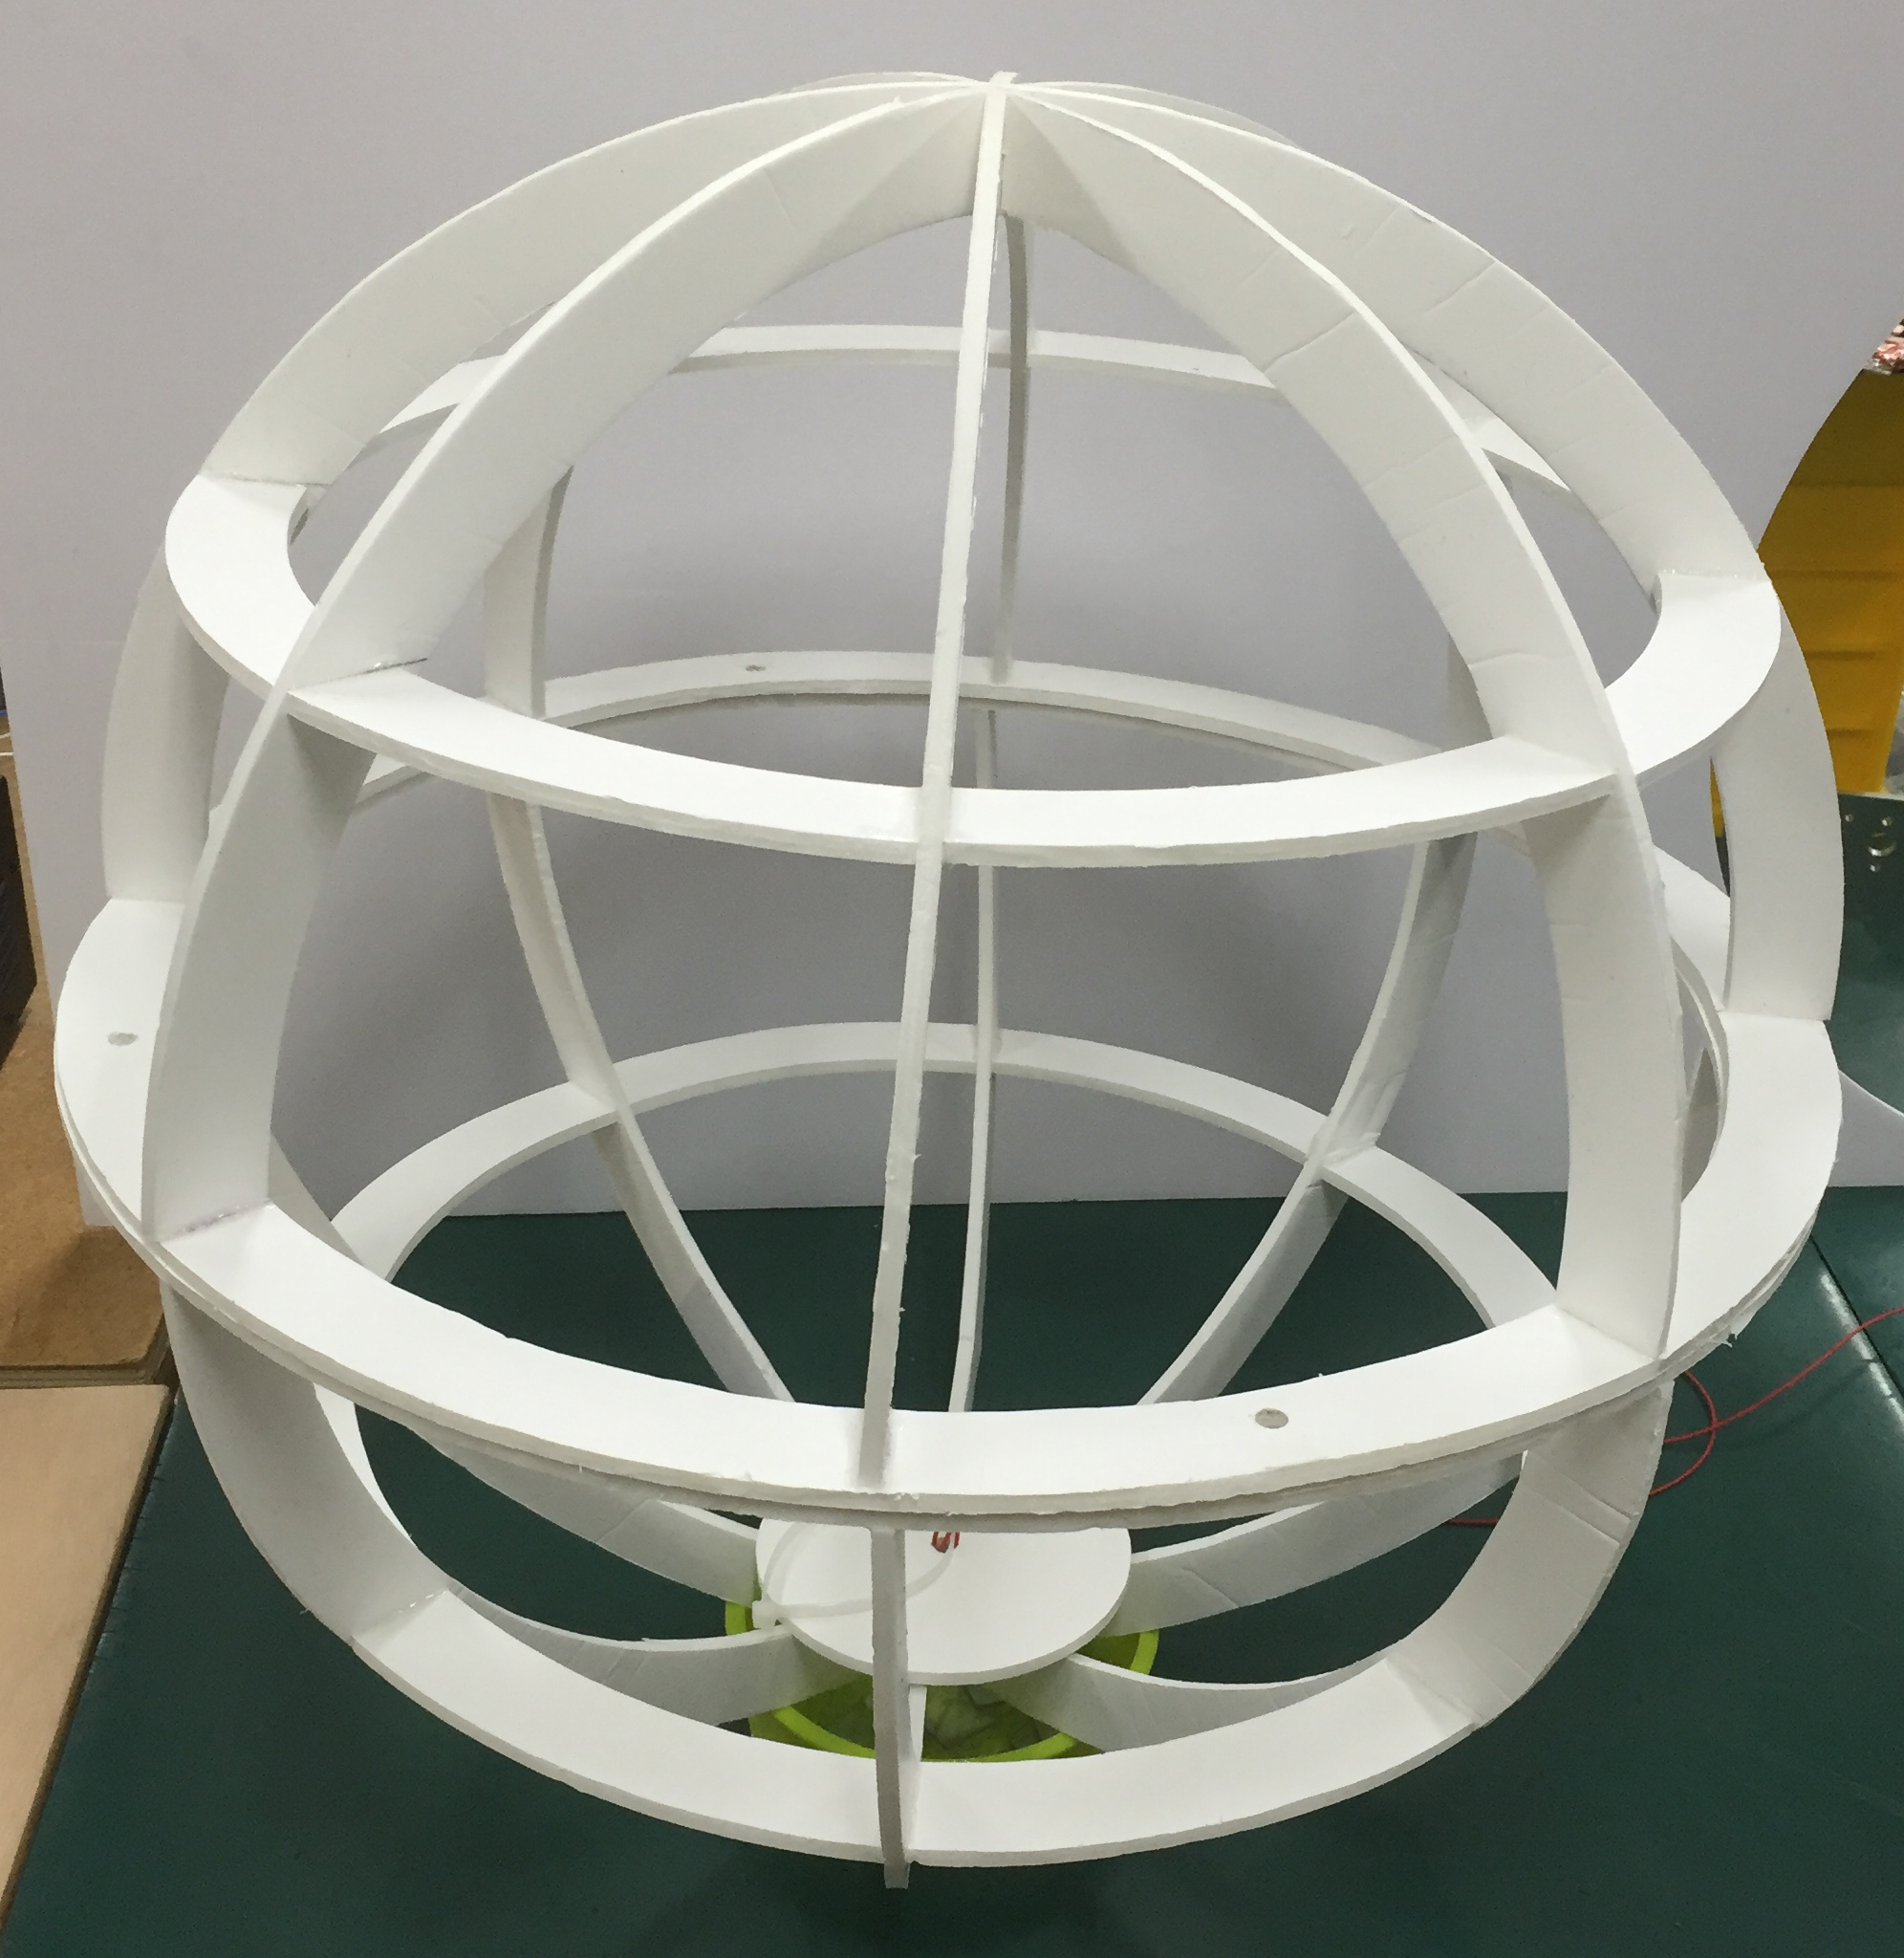
\includegraphics[width=50mm]{image/sphere-1.JPG}
  \caption{球体1号機}
  \label{fig:sphere-1}
 \end{center}
\end{figure}

\subsubsection{2号機}
1号機の構造ではスチレン材と紙が剥離してしまうので,Fig.\ref{fig:kigumi}のように極力木組み構造で組み立てるように変更した.
製作した球体2号機をFig.\ref{fig:sphere-2}に示す.

\begin{figure}[htbp]
 \begin{center}
  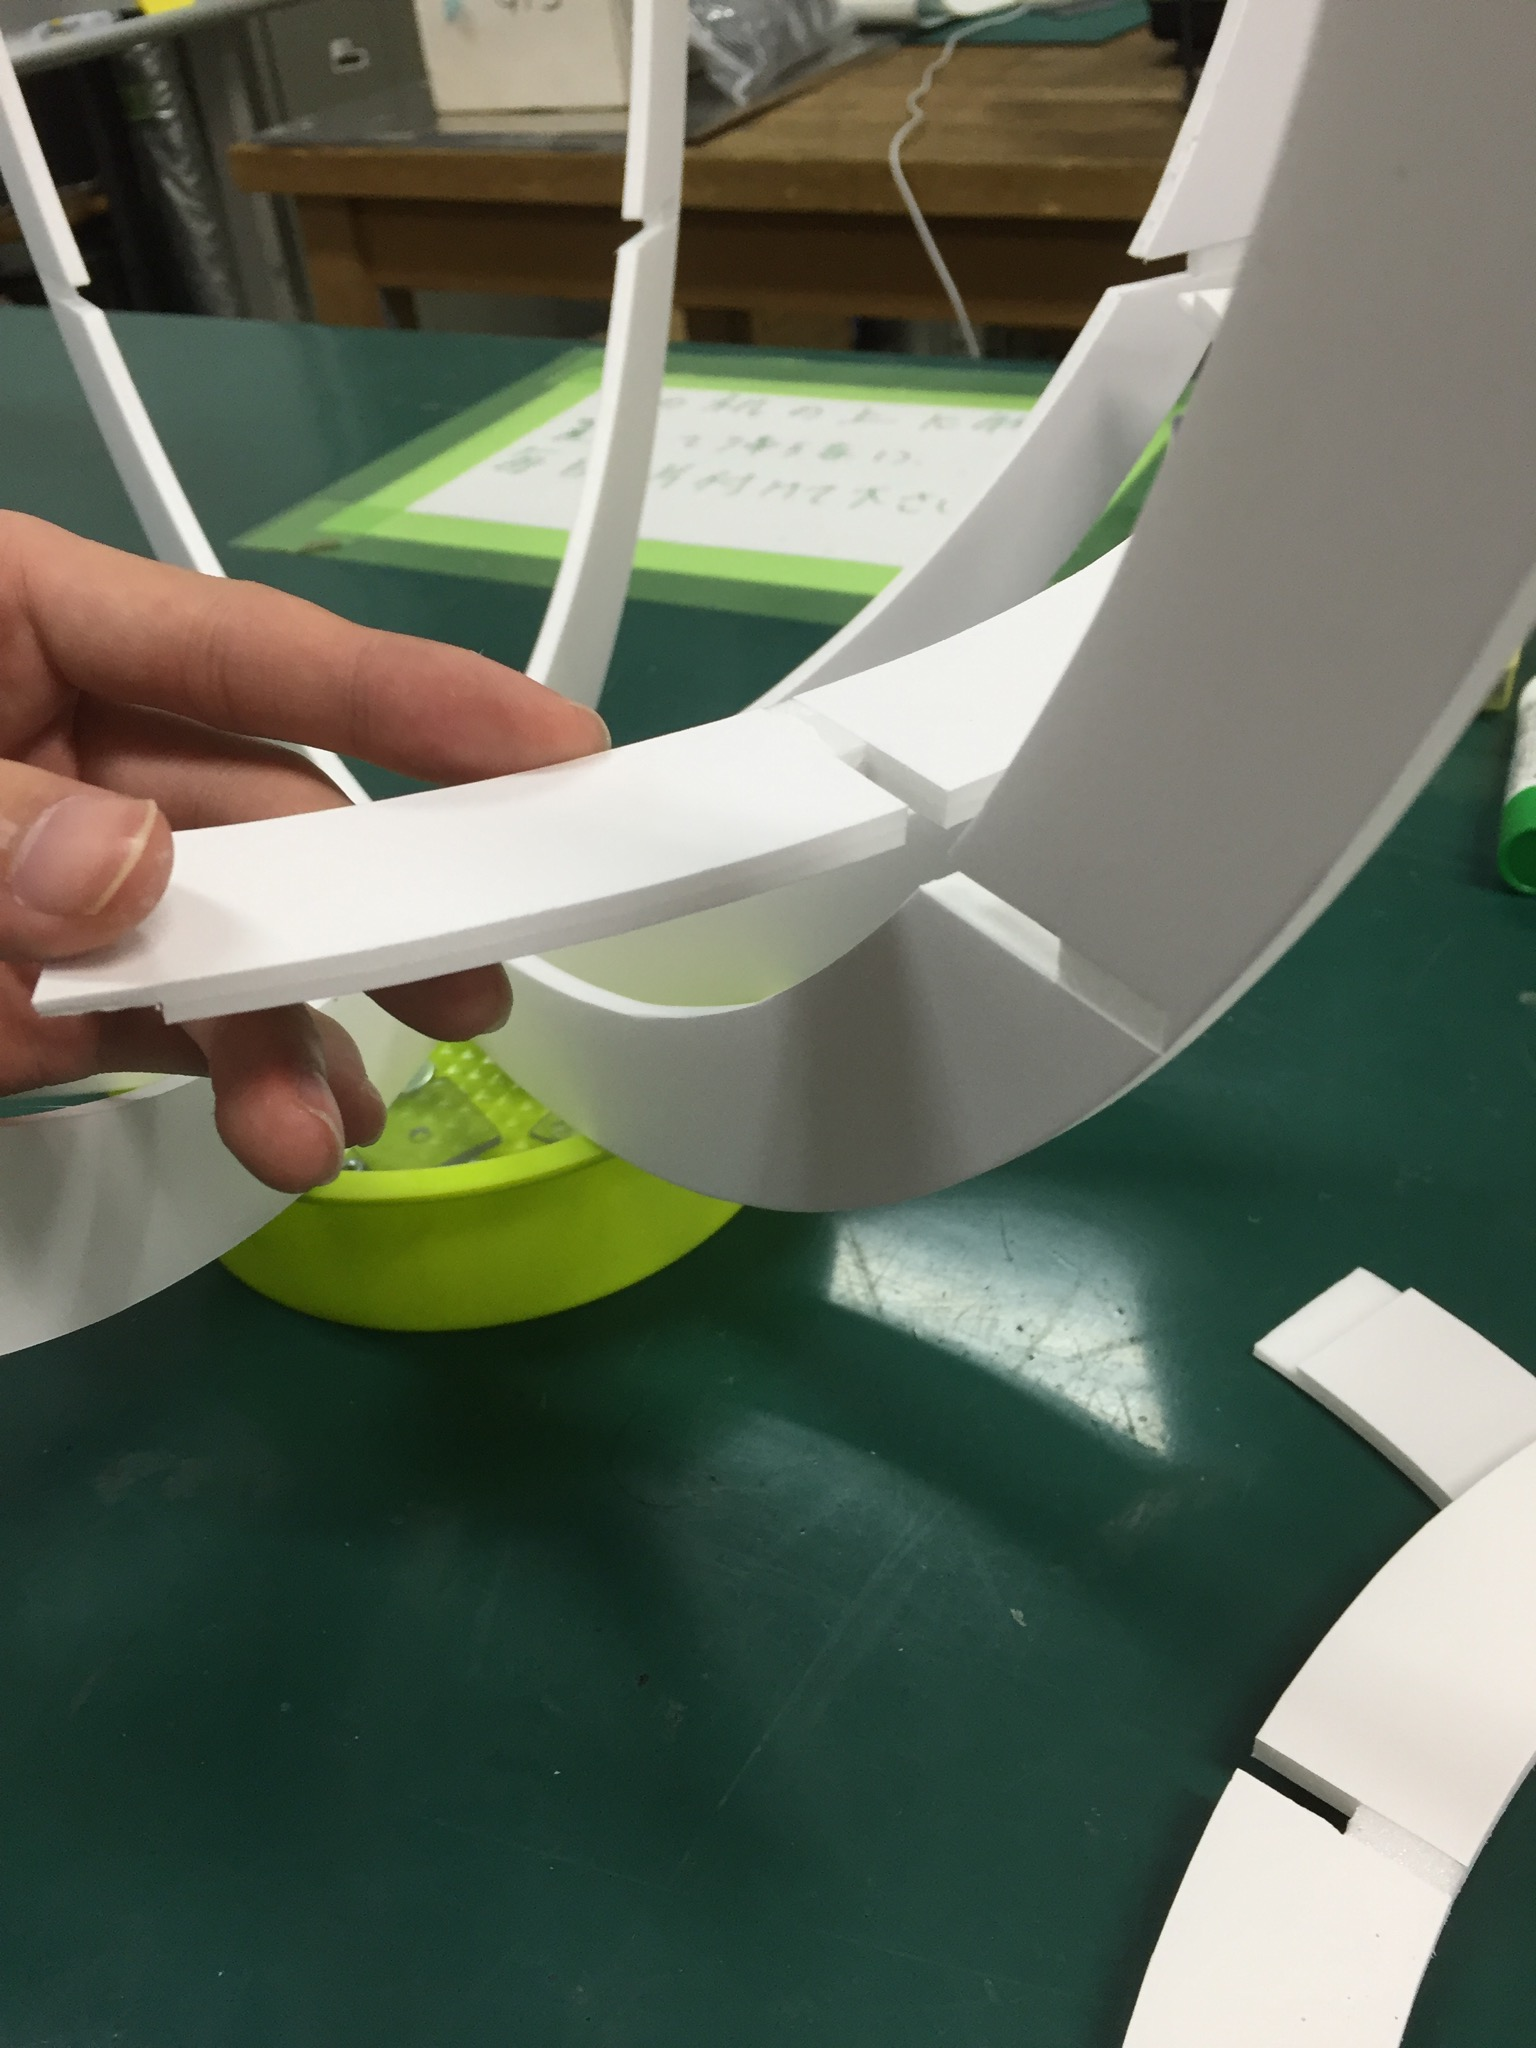
\includegraphics[width=50mm]{image/kigumi.JPG}
  \caption{木組み部分}
  \label{fig:kigumi}
 \end{center}
\end{figure}

\begin{figure}[htbp]
 \begin{center}
  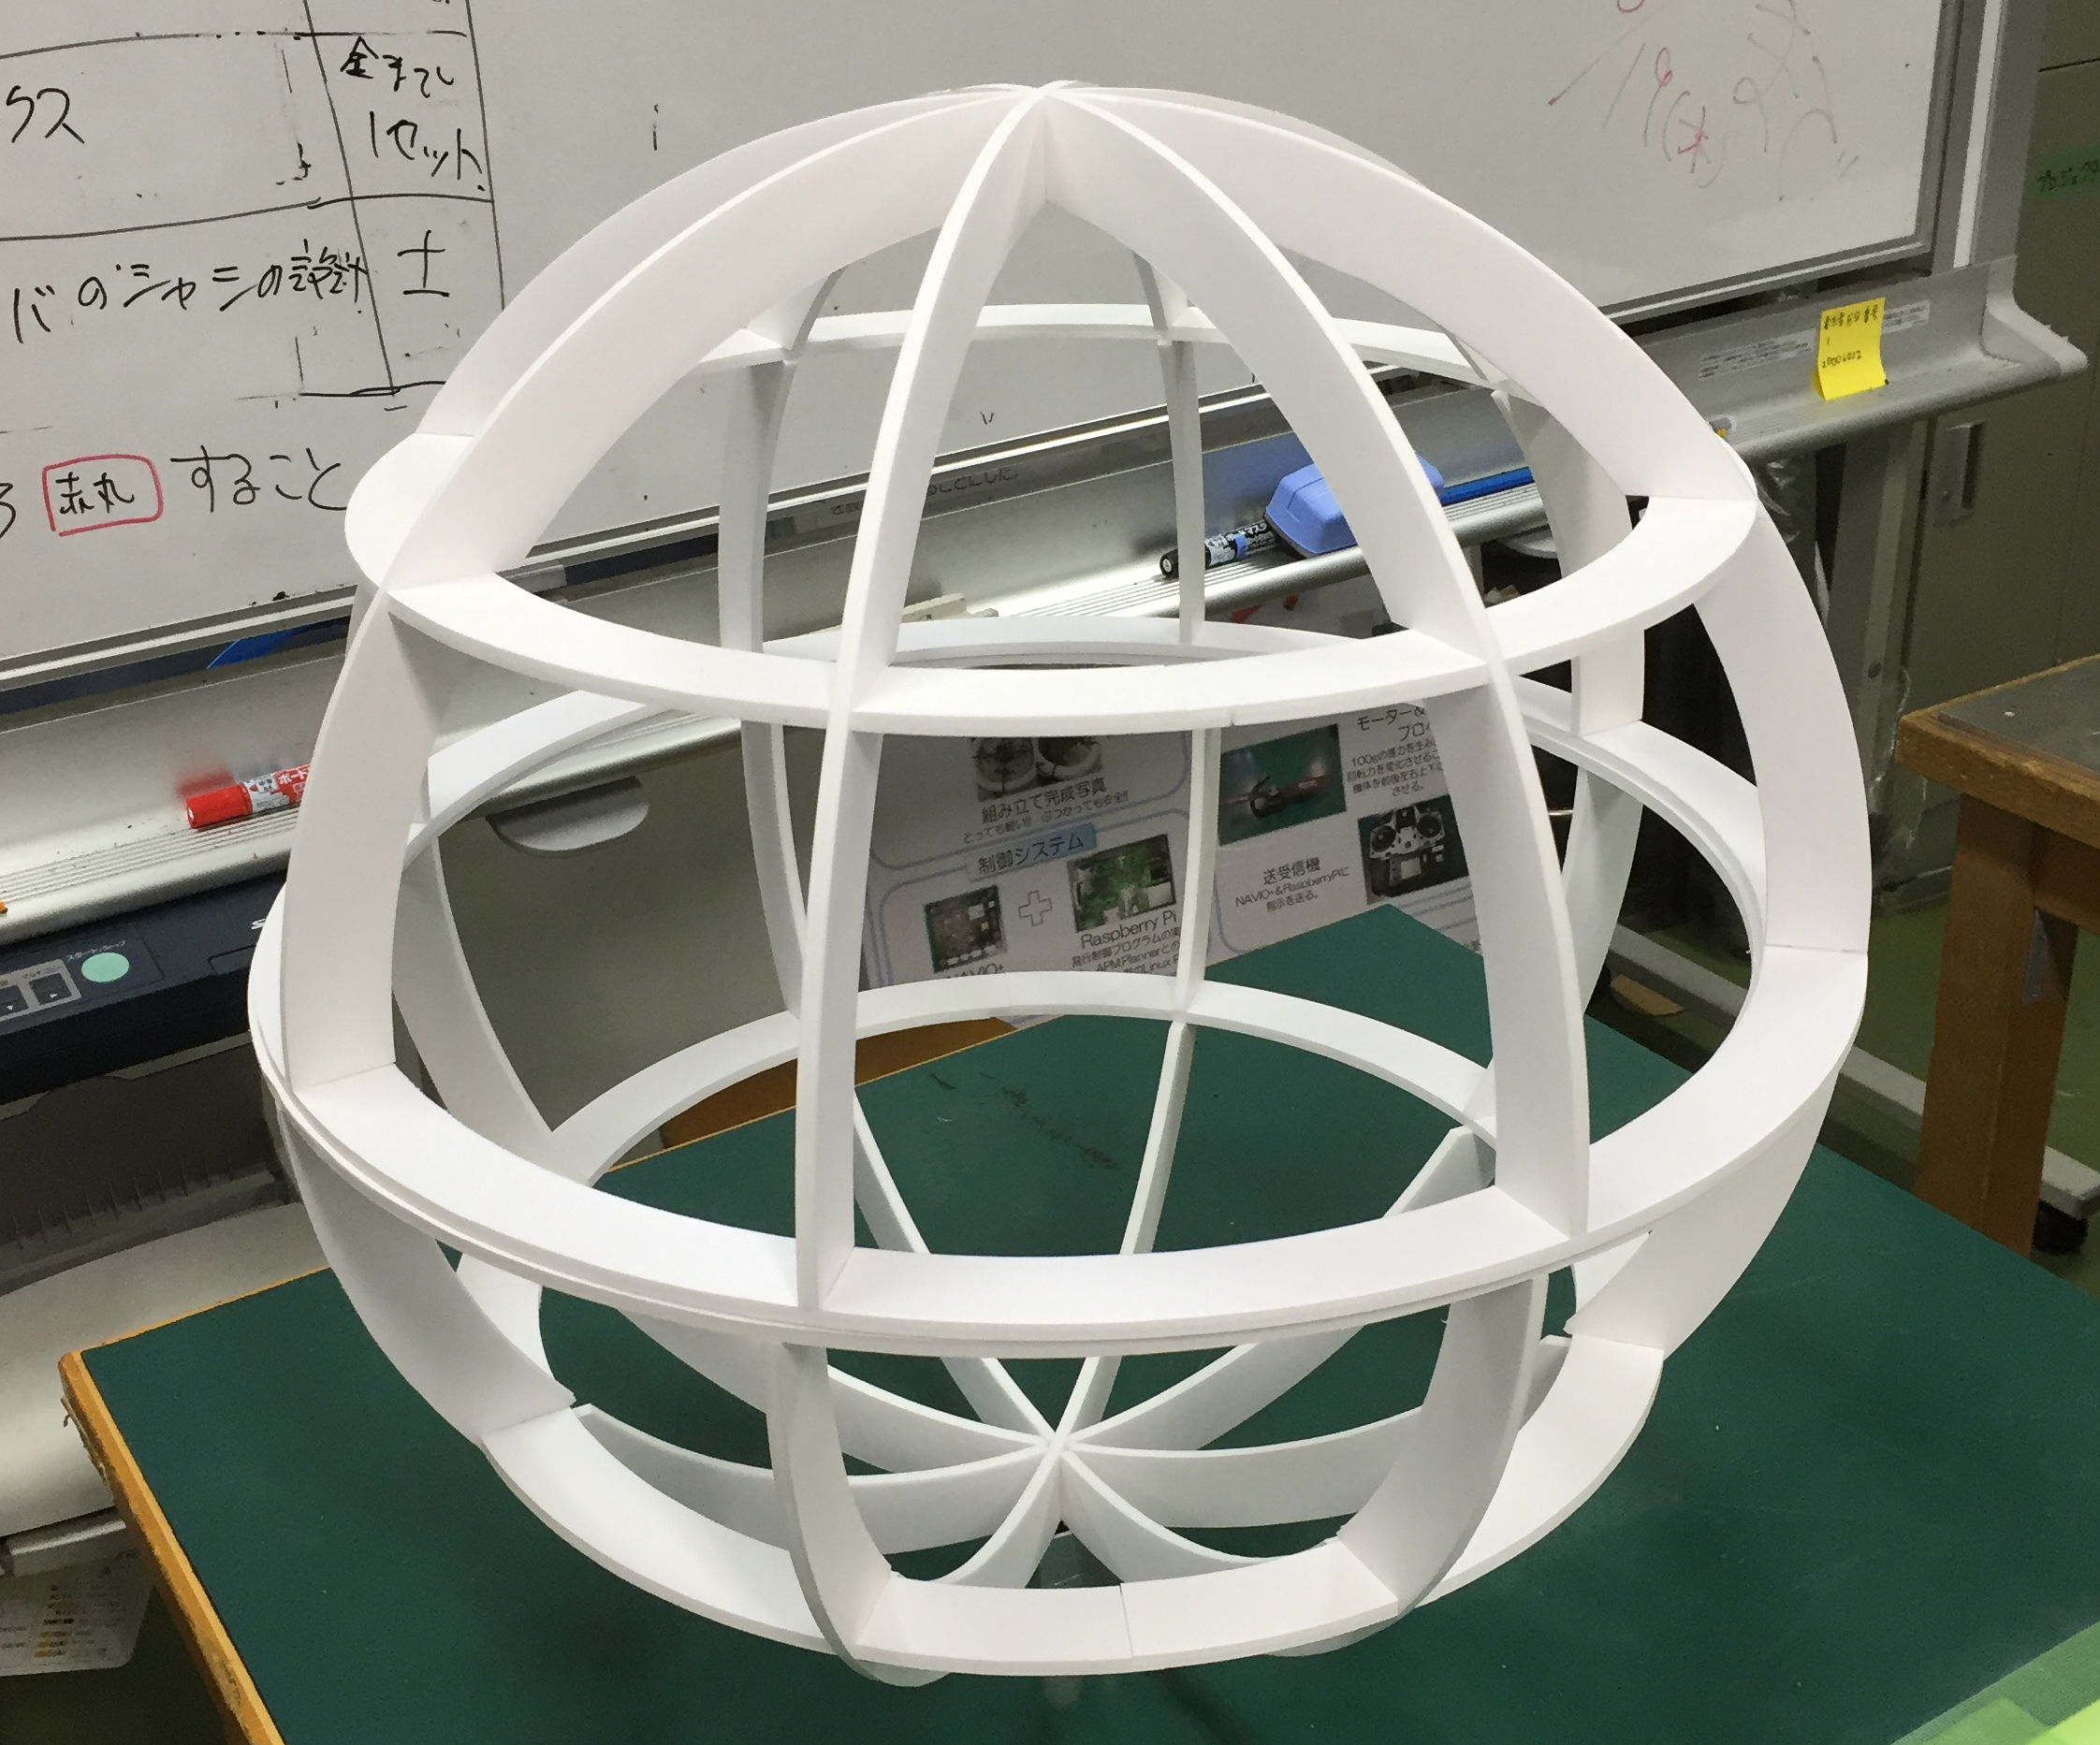
\includegraphics[width=50mm]{image/sphere-2.JPG}
  \caption{球体2号機}
  \label{fig:sphere-2}
 \end{center}
\end{figure}

\subsubsection{3号機}
1号機や2号機のように手作業で加工する場合球体1機の製作にとても時間がかかってしまため,スチレンボードの加工をレーザー加工機で行うことにした.
しかし,レーザー加工機で加工する場合,切断面のスチレン材がレーザー光の熱により溶けて凹むことが判明した.
接着のためには広い接着面積が必要なので,接着面以外をレーザー加工機で加工し接着が必要な部分を手作業で加工することにした.
製作した球体3号機をFig.\ref{fig:sphere-3}に示す.

\begin{figure}[htbp]
 \begin{center}
  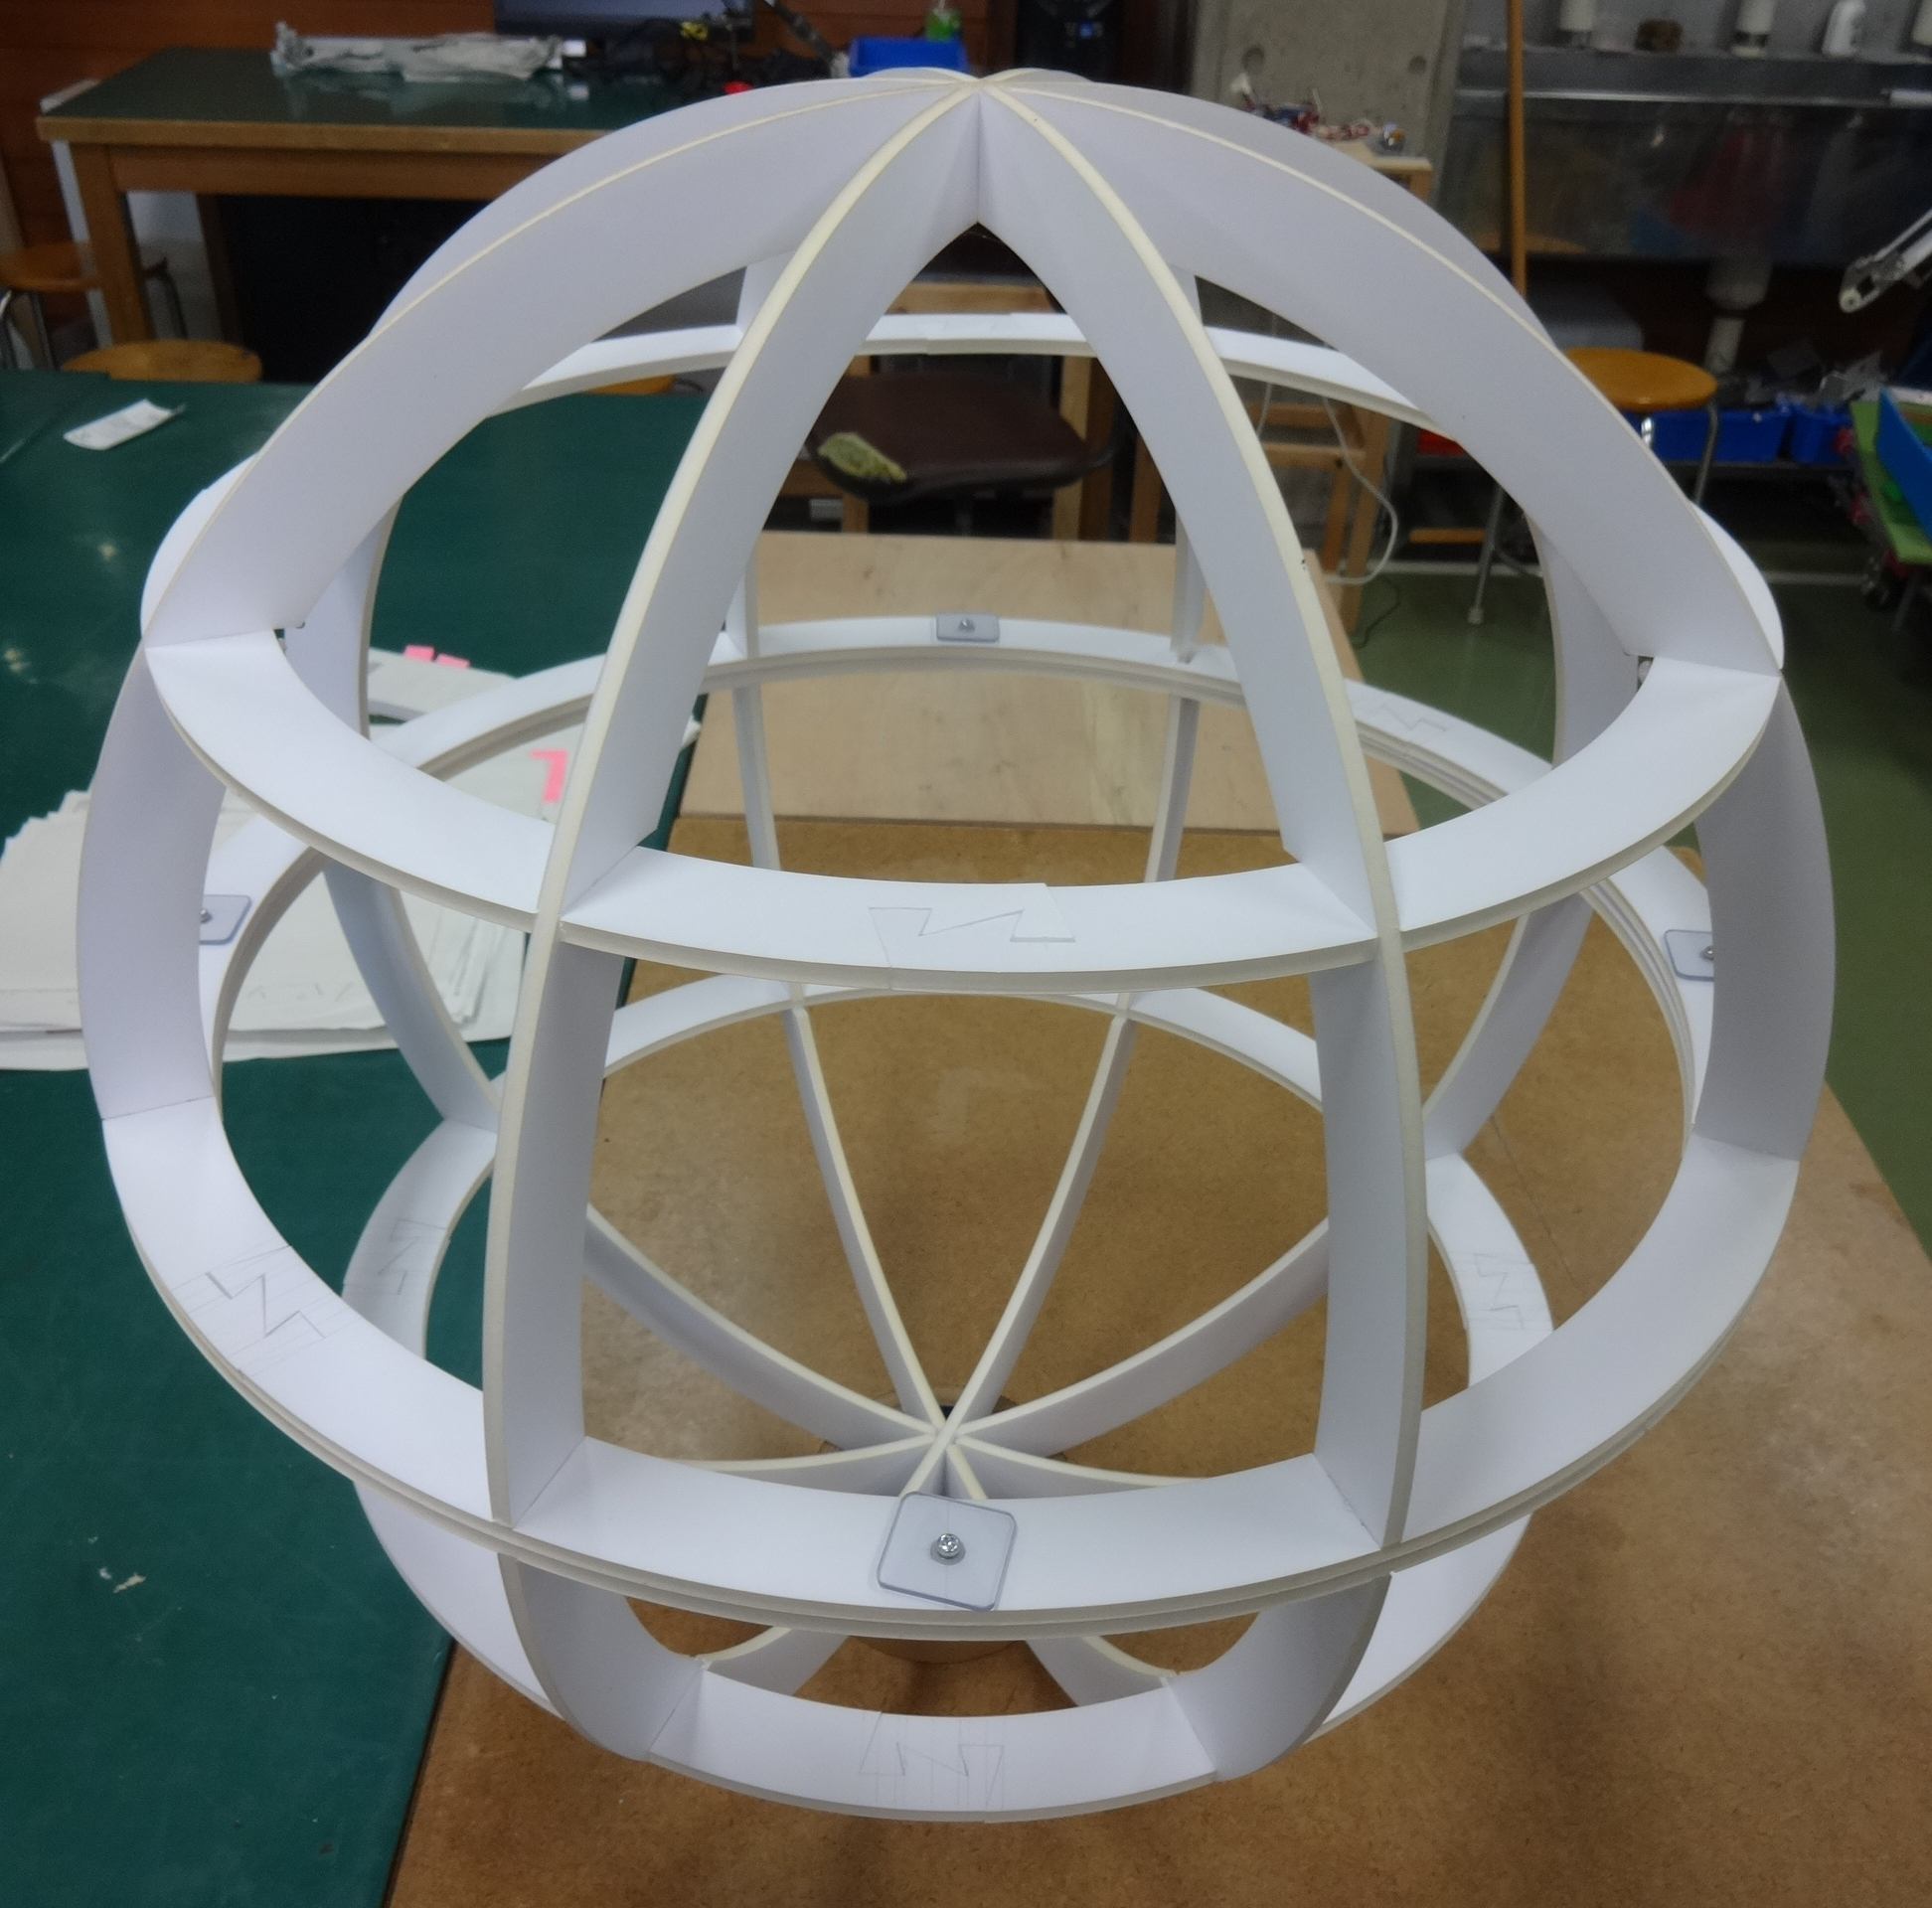
\includegraphics[width=50mm]{image/sphere-3.JPG}
  \caption{球体3号機}
  \label{fig:sphere-3}
 \end{center}
\end{figure}

\section{考察}
以上の結果から重量と強度を考慮すると,CFRPで試作2号機のようなコの字型のアームを交差させた形状を一体成型により製作することが望ましいと考えられる.
球体の材質にはプラスチックダンボールを使用するのが良いと考えられる.
プラスチックダンボールの性質としてFig.\ref{fig:cardboard}のように方向によって強度が違う.
そのため球体の上下部分に最も強度が高い部分を用いるように製作することで,スチレンボードでは足りなかった耐久性が改善できると考えられる.
球体はプラスチックダンボールで製作したことにより,落下時に最も強度が高い部分が当たるため壊れにくく目的に最も沿ったものとなったと考えられる.

\begin{figure}[htbp]
 \begin{center}
  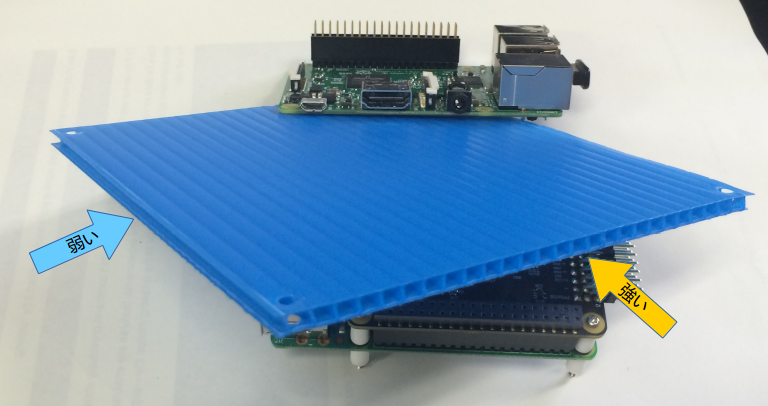
\includegraphics[width=50mm]{image/cardboard.png}
  \caption{プラスチックダンボールの特性}
  \label{fig:cardboard}
 \end{center}
\end{figure}

\section{ソフトウェア開発の目標}
目的の達成のためには自律飛行とマルチコプター間の通信制御が必要である.
マルチコプターの自律飛行にはPID制御を用いて飛行を行い,画像処理による3次元復元と3次元マッピングにより自己位置推定などを行う.
マルチコプター間の通信にはRPiを無線LANアクセスポイントとして用いることができるため,この機能を利用しての全マルチコプターを1つのネットワークに接続させて通信を行う.

\subsection{PID制御}
自律飛行を成功させるには,マルチコプターが安定して飛行できる必要がある.
そのため本研究ではPID制御を用いて飛行を安定化させる.
PIDとは比例(Proportional),積分(Integral),微分(Differential)の英語の頭文字をとったものである.
目標値に対し,制御偏差に比例した値,せいぎょへんさにを積分した量,および制御偏差を微分した量を加えあわせたものを操作量とする制御法である.[1]

\subsection{コントローラー}
本研究では,最終的には自律飛行を行うが制御が安定するまでの間コントローラーを使用して操作を行いゲインの調整などを行った.
コントローラーには,RPiにBluetoothモジュールが搭載されているためBluetooth通信が可能なゲーム用コントローラDUALSHOCK3を用いた.
コントローラーの右スティックをスロットルとヨー方向の制御に割り当て,左スティックをロール方向とピッチ方向の制御に割り当てた.
新しい機能が思いついた場合,使用していないボタンに機能を割り当てることができる.

\section{ソフトウェア開発の経緯}

\subsection{自律飛行に至るまで}
自律制御を行う前段階として,DUALSHOCK3をBluetoothでRPiに接続しマルチコプターの操作を行う.
本研究におけるマルチコプターの座標系とモーターの回転方向を示したものをFig.\ref{fig:config}に示す.

x,y,z軸それぞれの回転をx軸がロール,y軸がピッチ,z軸がヨーと呼び,それぞれ右ネジの回転方向を正とする.
Navio2のセンサから得られる情報から,ロール・ピッチ・ヨー方向のPID制御を行いマルチコプターの動作を制御する.
このPID制御の結果を用いて自律飛行に繋げる.

\begin{figure}[htbp]
 \begin{center}
  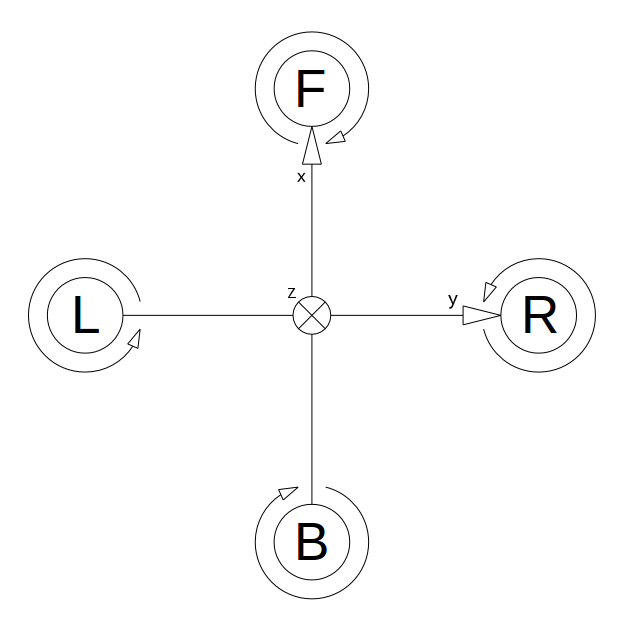
\includegraphics[width=50mm]{image/config.png}
  \caption{マルチコプターの設定}
  \label{fig:config}
 \end{center}
\end{figure}

\subsection{画像処理プログラムや音声認識プログラム}
同研究室で開発したプログラムを搭載した.
RPiの処理速度が遅いため画像処理プログラムがうまく動作しなかった.
音声認識プログラムはマルチコプターが駆動していない間はうまく動作していたが,マルチコプターの駆動音がノイズとなりうまく動作しなかった.

\section{考察}
機体を球体に入れたことにより,足をつけていた時より離着陸時の安定性が低下した.
離着陸時モーター特性の差から現在のプログラムでは水平を保とうとして発散してしまう.
今後,起き上がりこぼしの数式モデルを作成しプログラムに組み込むことでこの問題を解決できるのではないかと考えられる.

画像処理プログラムはRPiでも動作するライト版を開発することが求められる.
音声認識プログラムはノイズの除去機能を別途で開発することが求められる.

\section{おわりに}
マルチコプターを球体で覆うことにより,今までにない新規性が得られたと考えられる.
また、球体で覆ったことによりマルチコプターのプロペラで人を傷つけるような事故が減り,壁などにぶつかった時マルチコプター本体が破損しにくくなると考えられる.

今後の改善点として,機体の構造の簡易化やなどが挙げられる.
現在の形状は軽量であり強度は十分なのだが組み立てがしづらくメンテナンス性が悪いことが挙げられる.
そのため現在と同じくらいの強度を保ちながら組み立て易い構造に変更すべきである.

\section{参考文献}
[1]森泰親,"演習で学ぶPID制御",60,森北出版株式会社(2009)
%%%%%%%%%%%%%%%%%%%%%%%%%%%%%%%%%%%%%%%%%%%%%%%%%%%%%%%%%%%%%%%%%%%%%%%%%%%%%%%%

\end{document}
